\subsection*{SAR: MFP and \% Inhibition HCT-116}
\begin{figure}[htbp] % 'h' places the figure approximately here
    \centering
    \hspace{-1cm}
    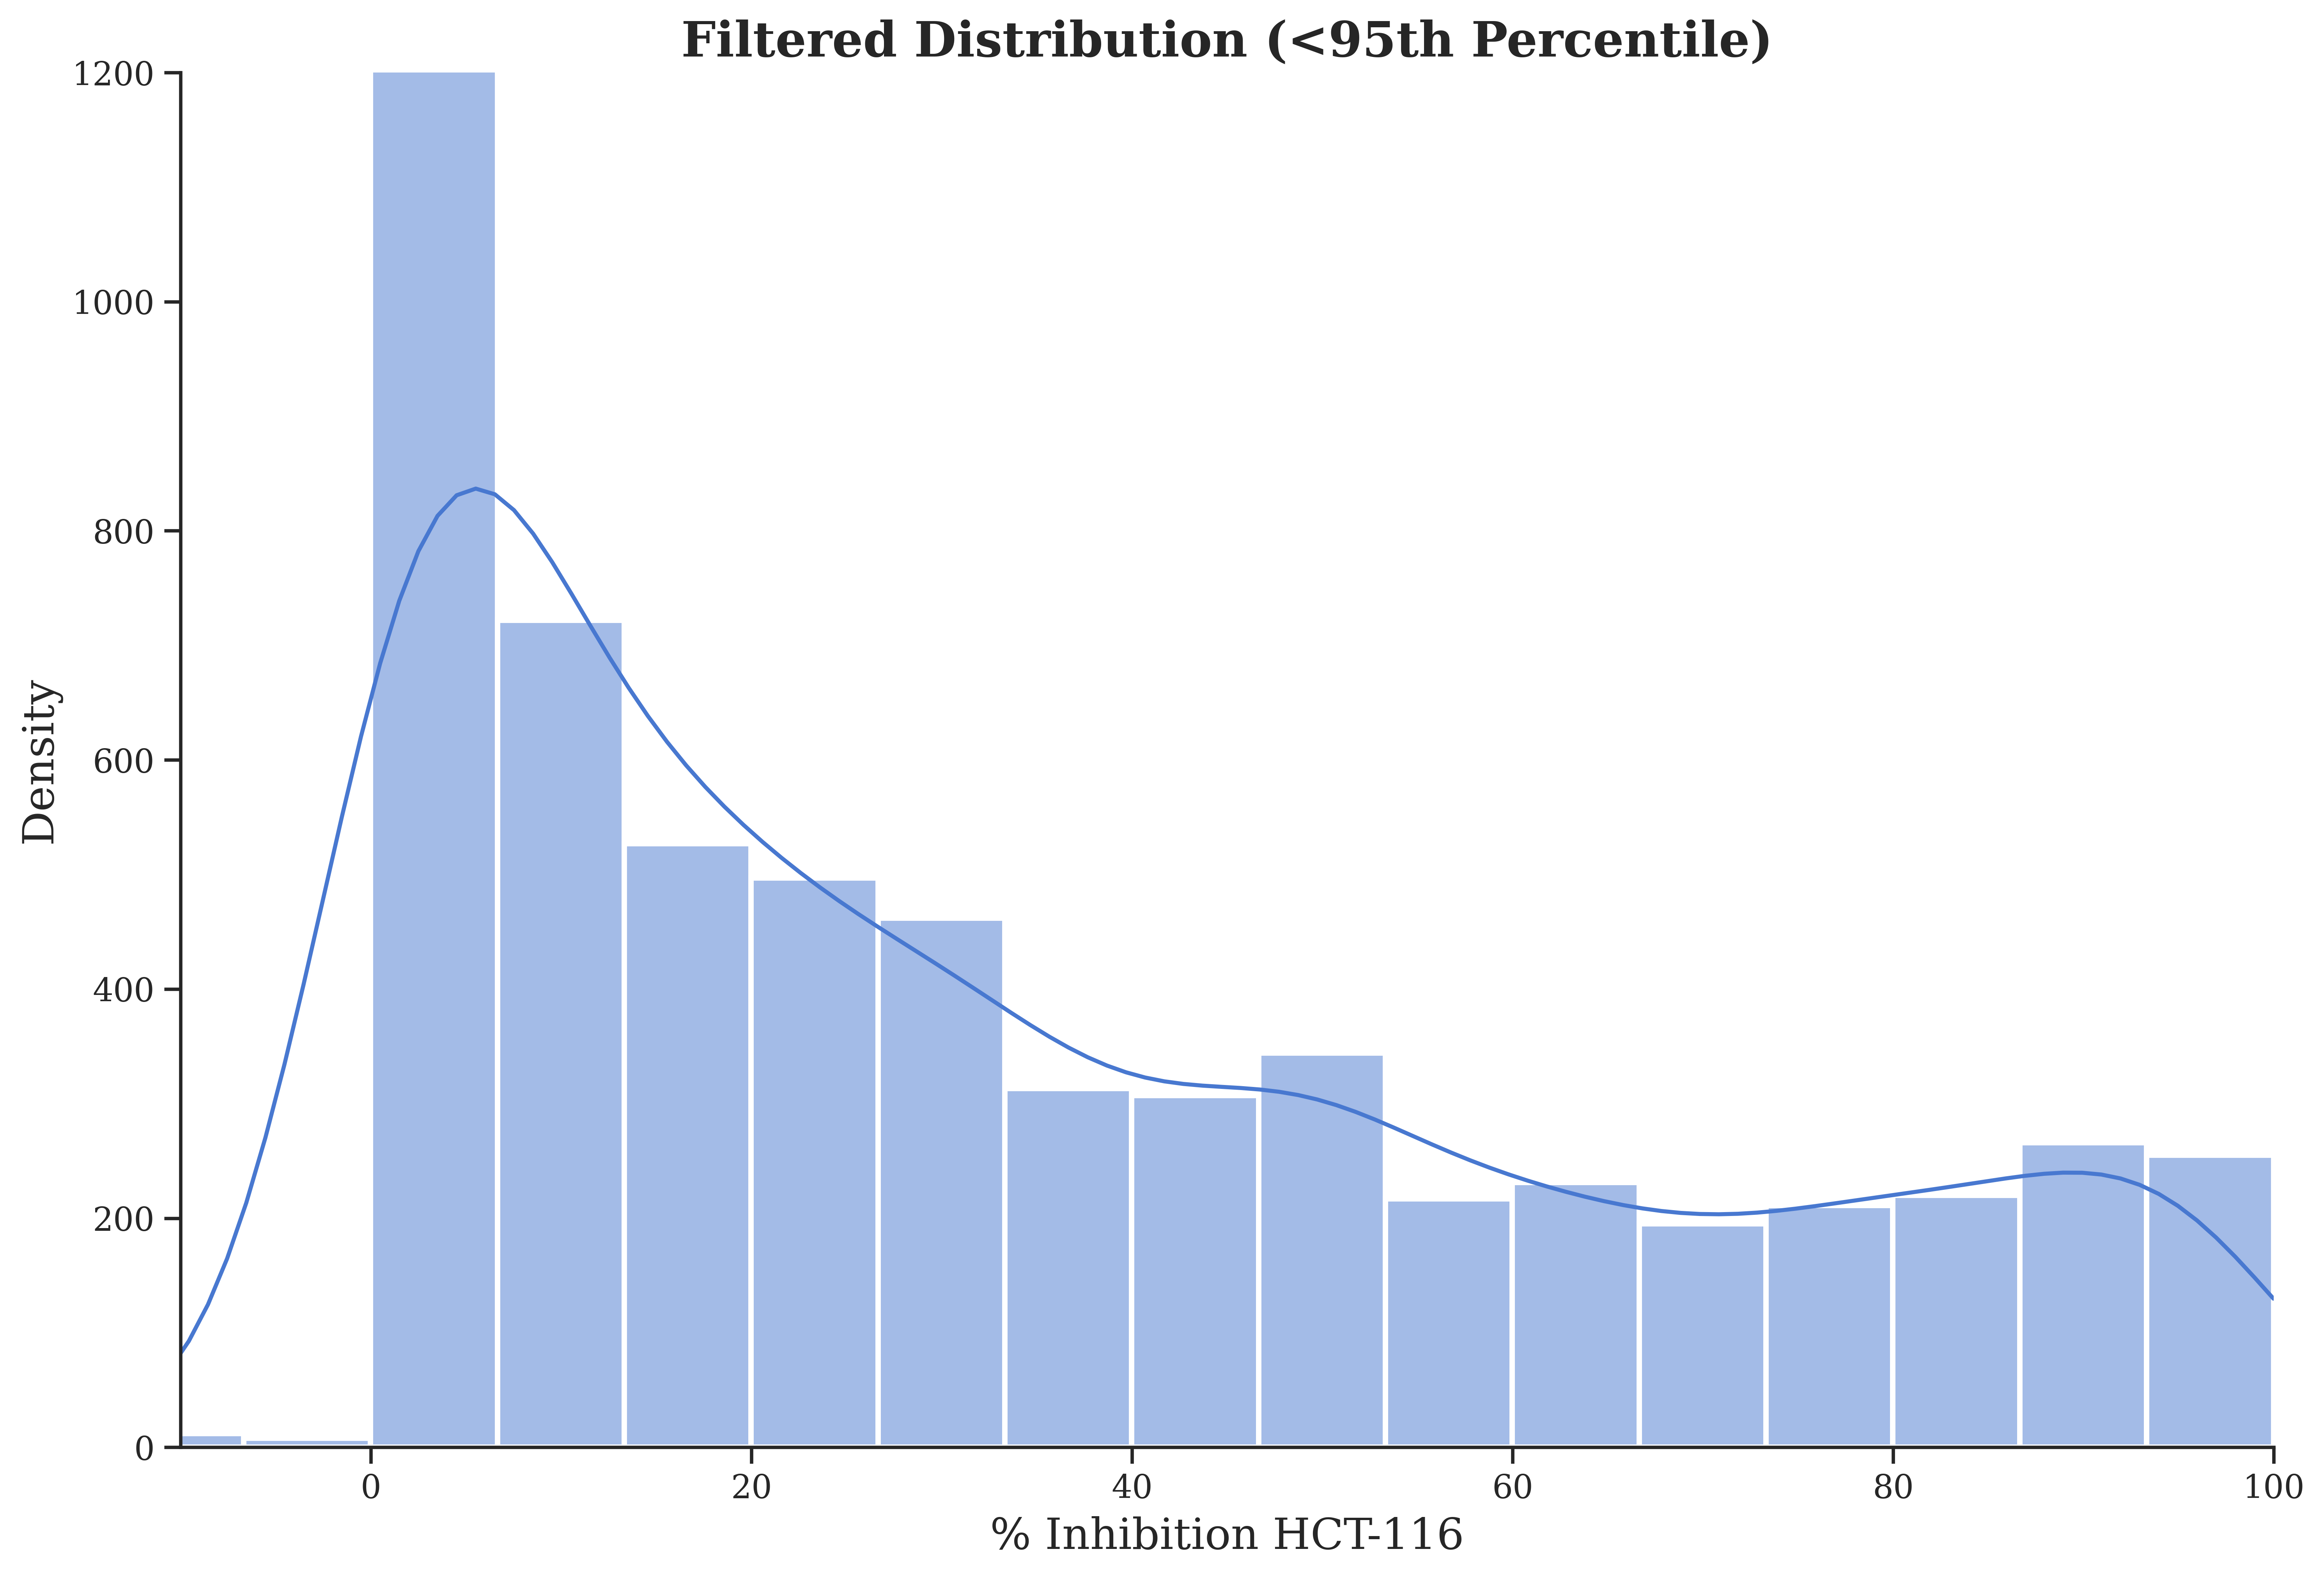
\includegraphics[scale=0.5]{cleandatadist.png}% Replace with your image filename
    \caption{Distribution of Cleaned Data Set of HCT-116}
    \label{fig:cleandist} % Optional: use \label for referencing
\end{figure}

Development of ML models are heavily dependent on the data quality \cite{zhou2024dataquality}. Erroneous and misleading predictions generated by the models were often associated to outliers that were not removed during the training and testing period. Unfiltered data set were observed to have 70.16 skewness, which means that most of the data outliers are located on the positive tail end of the curve. And If not removed, it is expected that the model out of it will produce positive errors. Thus, the data set used in this study were pre-processed prior to modeling, and the result shows that filtered data have skewness of 0.05386, suggesting a significant improvement in distribution. \autoref{fig:cleandist} shows that filtered/cleaned data has asymmetric normal distribution (i.e., imbalanced data set). SMOTE results to balanced the minority and majority class of the data set, thus, removing positive biases in models predictions (\autoref{fig:SMOTE}).

\FloatBarrier
\begin{figure}[h]
	\centering
	\begin{minipage}{\textwidth}
		\centering
		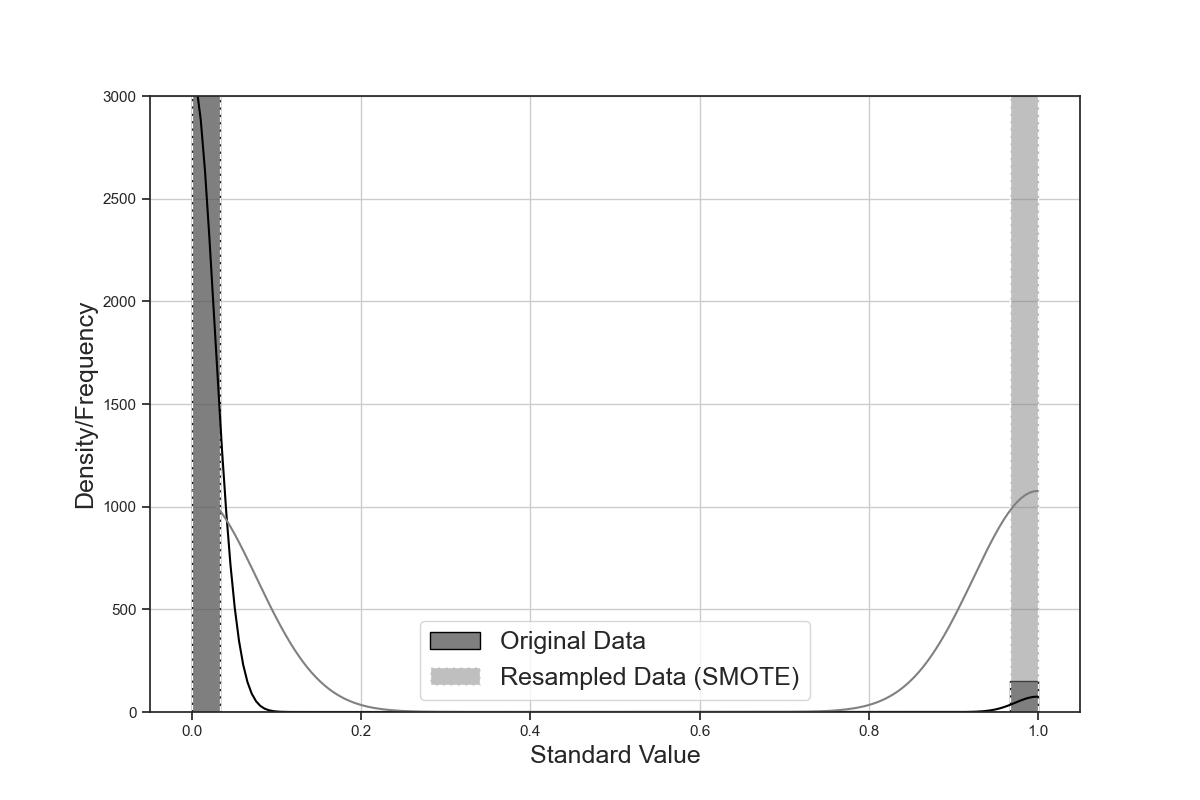
\includegraphics[width=1\textwidth]{SMOTEbw.png}
		\vspace{-1cm}
		\caption{Comparison of Distributions Before and After SMOTE}
		\label{fig:SMOTE}
	\end{minipage}
\end{figure}
\FloatBarrier

%\begin{figure}[htbp] % 'h' places the figure approximately here
    %\centering
    %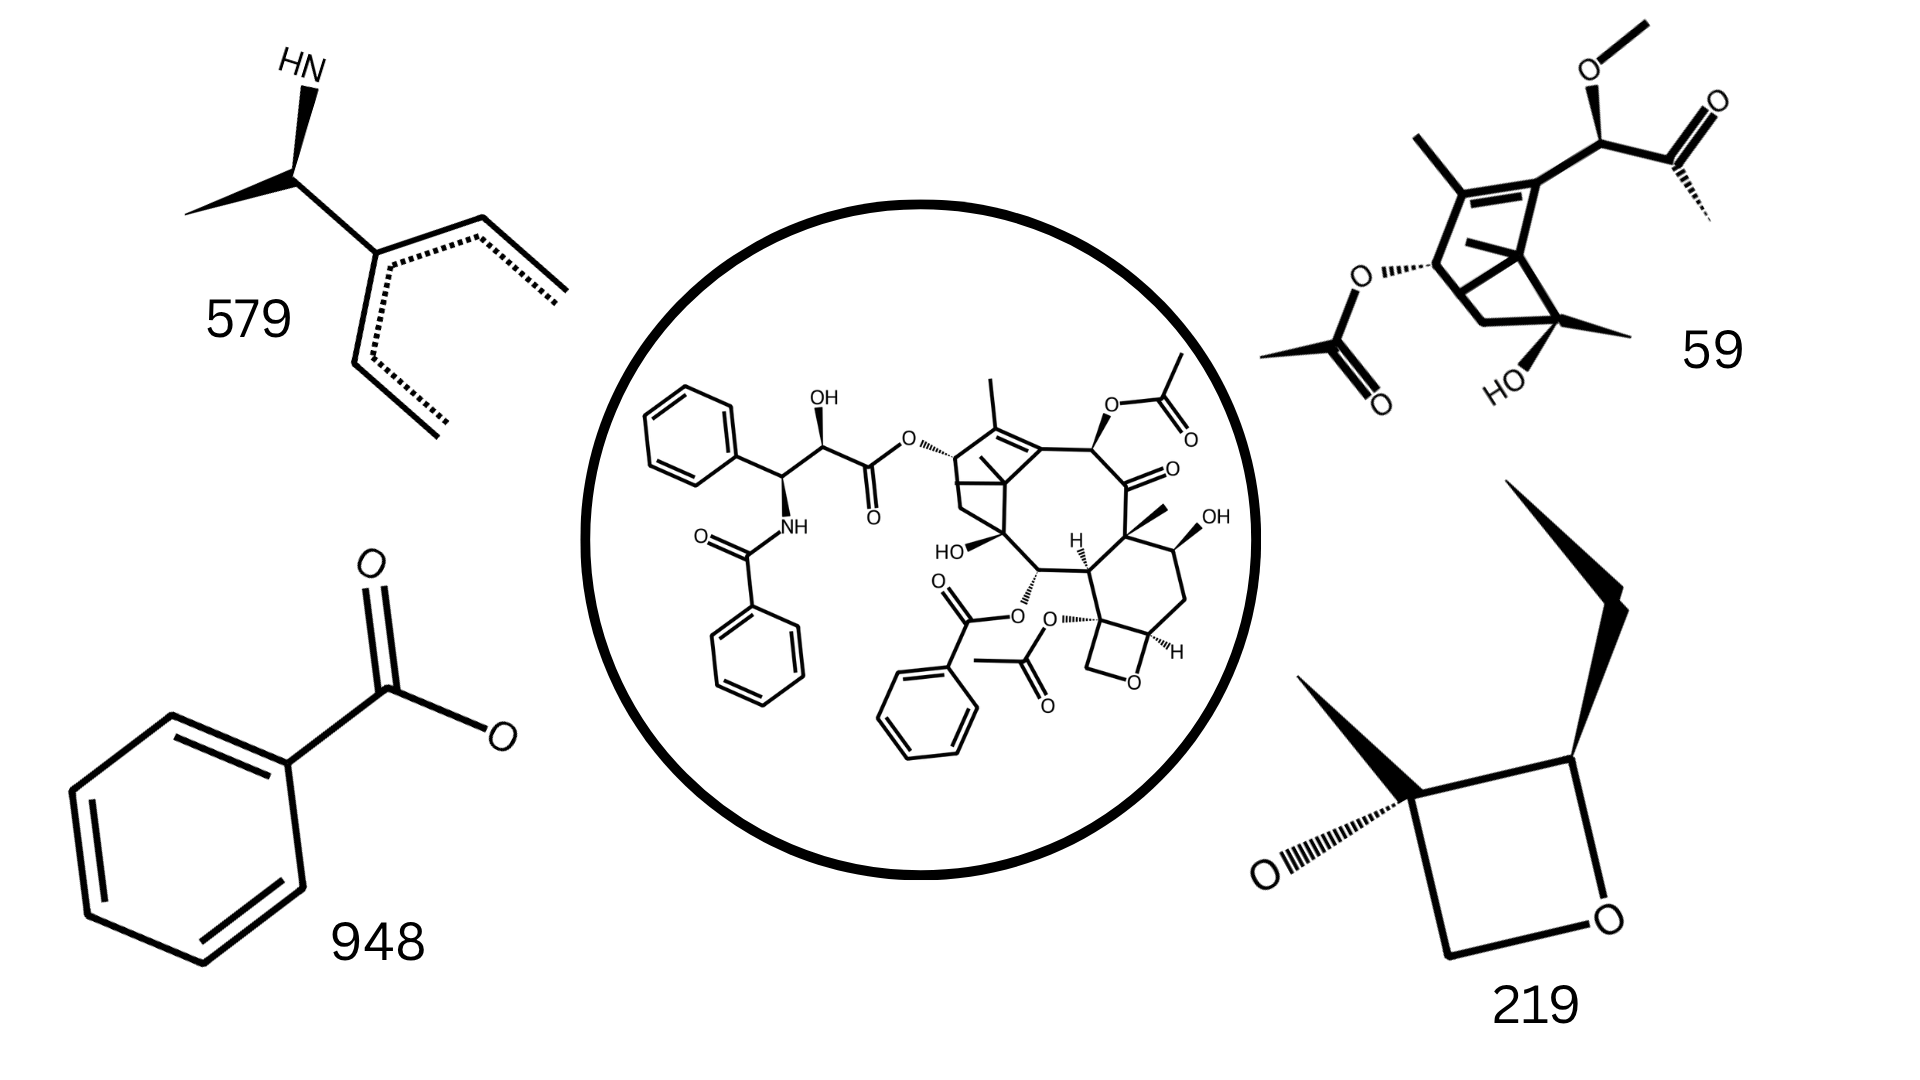
\includegraphics[width=0.7\textwidth]{fragmentation.png}% Replace with your image filename
    %\caption{Fragmentation of Target Compound to Produce MF and Bit Number Assignment}
    %\label{fig:mfex} % Optional: use \label for referencing
%\end{figure}

The MFA produce a maximum of 2048 bits for each compound, and a total of approximately 12 million bits were analyzed in this study. \autoref{tab:summary} presents the summary of pre-processing, and generation of MF's and MP's through MFA. CBC method revealed that there are bits that were frequently present in molecules with or without bioactivity against HCT-116, Appendix A \autoref{tab:t10crude} shows the top 10 bits observed with CBC. Nearly all of the top 10 bits identified from CBC can be considered as small fragments. Changes in these bits could lead to positive or negative effects to molecules bioactivity against HCT-116 (\autoref{fig:top10crudebits}). Since the bits were not segregated and non-significant bits were not removed prior to bit frequency counting, thus, it is possible that the identified top 10 bits contain a mixture of positive, negative and non-significant bits. 
%To perform QSAR studies of the given clean data set, the generation of MF's plays the pivotal role on giving the MFA its capacity to perceived structural patterns in a binary format.  

%To gain a meaningful structural insight, the CBC and CSBC were employed. In essence, the presence and absence of particular bits and its relation to \% Inhibition can be simply detected by means of counting its frequency. This simple logic was leveraged in CBC method, wherein after the generation of MP's and MF's of the compounds, bit of a specific MF's were counted and ranked (see \autoref{tab:t10crude}). Essentially, the MF with highest bit frequency were expected to have a relationship with the \% Inhibition of compounds against HCT-116. On selecting the top 10 bits, researchers set the frequency values to at least 50\% of the total data, assuming that it is equal to the amount of observation that has a significance.

\begin{table}[h] % Optional: for floating the table
	\centering
	\begin{threeparttable}
		\renewcommand{\arraystretch}{1.2} % Adjust row spacing (1.2x normal)
		\small
		\begin{tabular}{p{3cm} p{4cm} p{4cm} p{2cm} p{2cm}} % Five columns (all centered and with vertical borders)
			\hline
			Molecule ChEMBL ID & SMILES & Mols \tnote{a} & \%Inhibition & MP \\ 
			\hline
			CHEMBL259084 & O=C(O)c1ccc$\ldots$ & rdkit.Chem.rdchem.Mol object at 0x00000225A15$\ldots$ & 6.400 & 111010101$\ldots$ \\ 
			CHEMBL224940 & CCCCN1CCN(C(=O)$\ldots$& rdkit.Chem.rdchem.Mol object at 0x00000225A15$\ldots$ & 27.000 & 101110100$\ldots$ \\ 
			CHEMBL2029910 & CN1CCN(C(=O)c2cc$\ldots$ & rdkit.Chem.rdchem.Mol object at 0x00000225A15$\ldots$ & 0.003 & 101010100$\ldots$ \\ 
			\vdots & \vdots & \vdots & \vdots & \vdots \\
			CHEMBL3813873	 & FC(F)(F)c1ccc$\ldots$ & rdkit.Chem.rdchem.Mol object at 0x00000225A16$\ldots$ & 4.280 & 111110101$\ldots$ \\ 
			\hline
		\end{tabular}
		\begin{tablenotes}
			\item[a] Mols indicates molecular object data type which is interpret as display or png file by rdkit package. 
		\end{tablenotes}
	\end{threeparttable}
	\caption{Summary of Compounds Data Profile}
	\label{tab:summary}
\end{table}

 \begin{figure}[htbp!] % 'h' places the figure approximately here
 	\centering
 	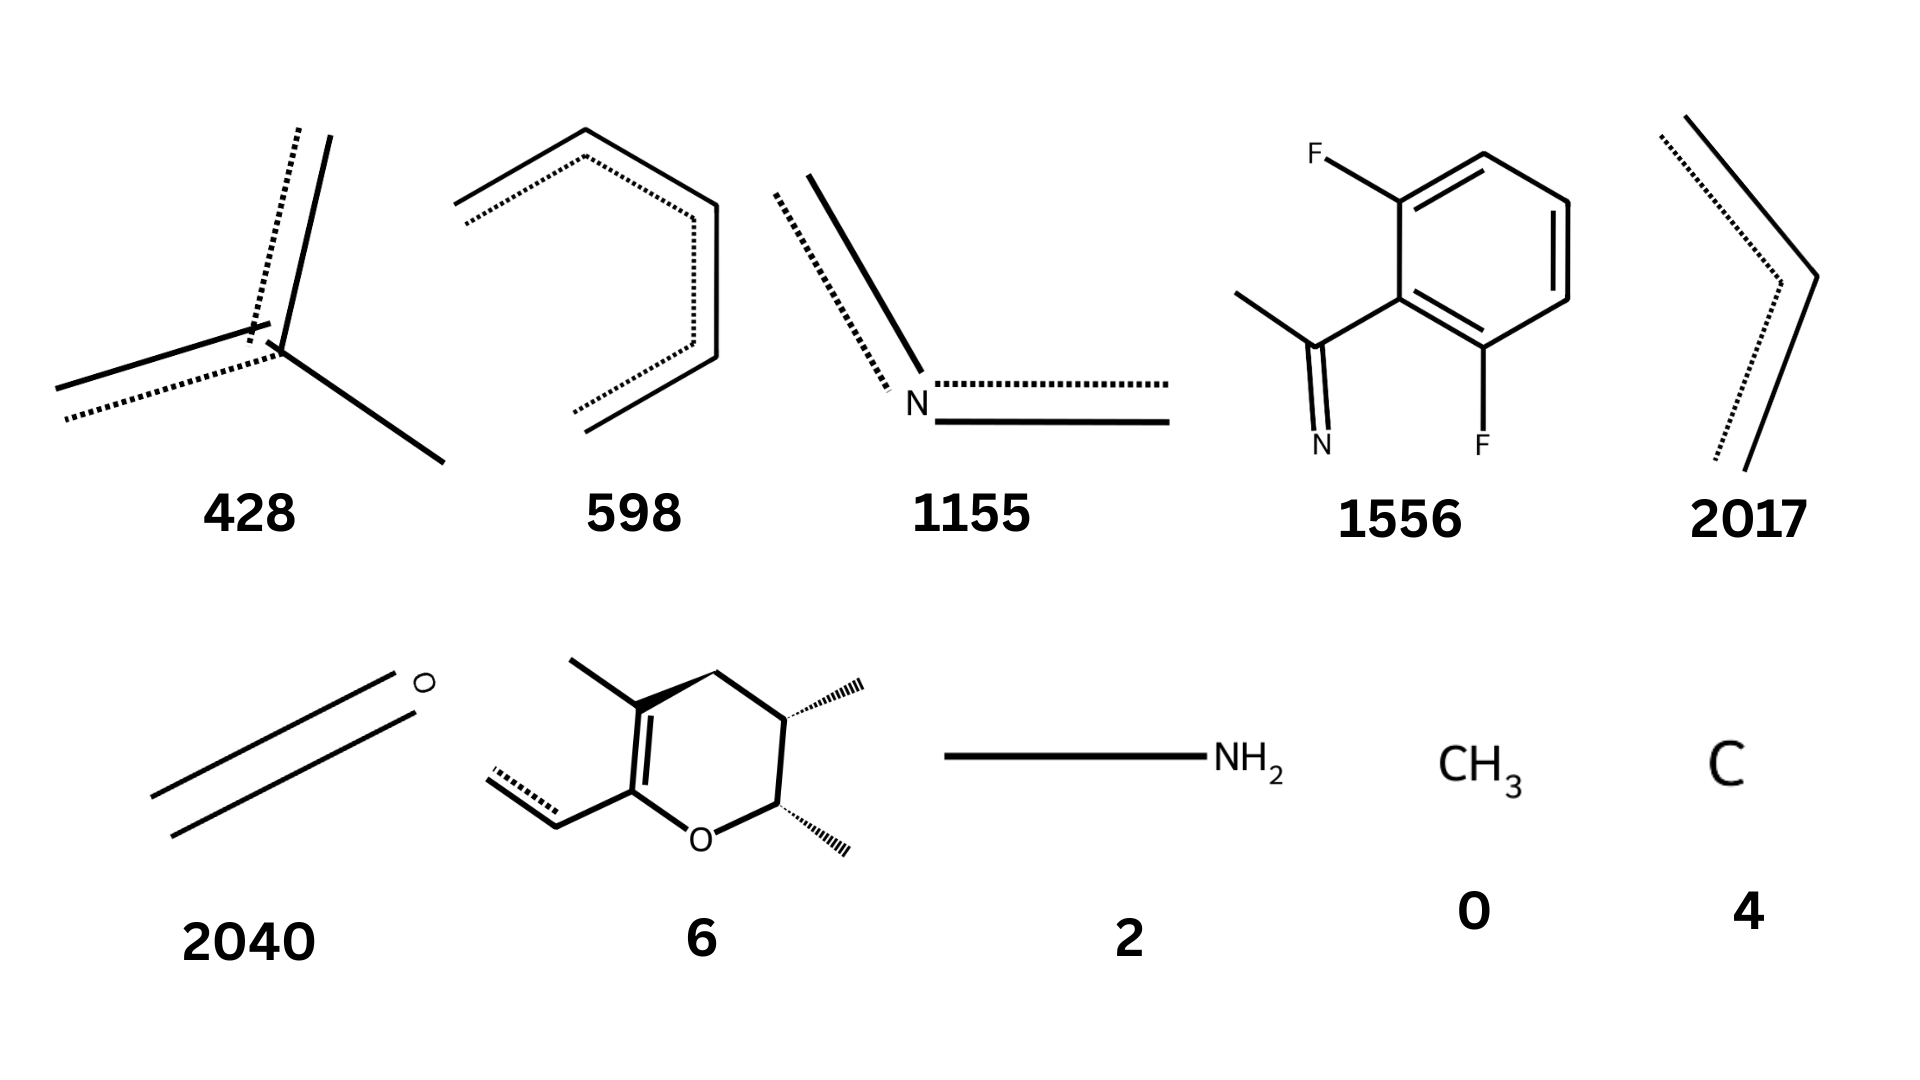
\includegraphics[scale=0.30]{top10crudebitsv2.png} % Replace with your image filename
 	\caption{CBC Top 10 Bits: 2D- Structures}
 	\label{fig:top10crudebits} % Optional: use \label for referencing
 \end{figure}
 
%Based on the results CBC identified the following bits: 0, 2, 4, 2017, 2040, 428, 6, 1556, 1155, and 598 as significant bits. Wherein, the algorithm suggest that these bits have a significant relationship with the bioacitivity of compounds. The machine 2D perception of the bits are quite unique, for it accounts the following: a) central atom (colored with blue dots); b) atomic substitution (color yellow)\footnote{yellow color represents sulfur substitution or other electronegative atoms}; and c) predicted bonds at the end of structure (colored with gray)\footnote{dashed grey line represents partial bonds}. Structurally, almost all of them were considered to be a small fragments, this could mean that structural or conformational changes in this bits could lead to inactivity of a compound (\autoref{fig:top10crudebits}). However, it was assumed that since the bits were not segregated and non-significant bits are not removed prior to bit frequency counting, probably the constituents of Top 10 bits from CBC could have a mixture of positive, negative and non-significant bits. To verify this assumption, the identified structural features will be used in the creation of CBC-ML, wherein the machine will be train and test to classify compounds activity based on the input features extracted from this method.  

CBC method is quite simple and might be a powerful technique to identify the significant bits from the clean data set, however, this method may not incorporate information on the position and neighboring structural motifs. Hence, it is possible that there will be cases that the presence or absence of a particular bit will have different meanings depending on their position or neighbor. In contrast, because CSBC employed blind clustering it allows for the segregation of data prior to counting. This intermediate  step gives an insight on the different clusters that exist in the given data set, which could lead to classification and discovery of new structural patterns. The assumption is that the common features shared among clusters will implicitly incorporate the dependency on position and neighborhood of structural motifs. Furthermore, subtraction of clusters  may naturally remove non-significant bits which could lead to more efficient identification of positively and negatively contributing bits. 

%several critical factors to understand and accurately classify the compounds based on their structural features. The researchers identified these critical factors to be the position and neighbor of bits. The algorithm used in CBC does not take into account where does the bits located and what are its neighbors during the counting process. Therefore, it is probable that there will be cases that the presence or absence of a particular bit will have different meanings depending on their position or neighbor. To mitigate this possibility, another method is developed to account these kind of scenarios which is called CSBC. In CSBC, blind clustering was first employed prior to counting, this was done to segregate the data sets and simplify it prior to counting. This intermediate step gives an insight about the different clusters that exist in the given data set that could lead to classification and discovery of new structural patterns. Essentially, the researchers assumed that, these clusters of compounds will have something in common and different, therefore, if these information could be extracted, probably the dependency in position and neighbors of the compounds could be understood. Furthermore, researchers also assumed that by doing blind clustering the presence of non-significant bits could be removed giving a way to identify early on the positive and negative bits. 

Result shows that the optimum number of clusters for the given data set using the Elbow Method is 5 (\autoref{fig:elbow}). K-Clustering divided 6304 \% Inhibition data into 5 categories which were classified as: a) HI (purple); b) MI (blue); c) LI (orange); d) VLI (green); and e) NI (red) (\autoref{fig:cluster}). The VLI region in \autoref{fig:cluster} contains the compounds with \% Inhibition of around -20 to 20, and it can be considered as the neutral point of the bioactivity \footnote{region of the data set that could be regarded as non significant bioactivity, close to 0 \% Inhibition}. The assumption is that structural features of compounds under that category could be non-significant and must be removed. In addition, it is also assumed that from the set neutral point going up and down to HI and NI respectively; may mean that alteration of molecules structures in that region might lead to maximization or minimization of bioacitivity against HCT-116. Therefore, subtraction of molecules MP in the VLI region from those  in the HI, MI, LI, and NI regions may lead to the extraction of structures that either increase or decrease their bioactivity.        

\begin{figure}[h] % 'h' places the figure approximately here
    \centering
    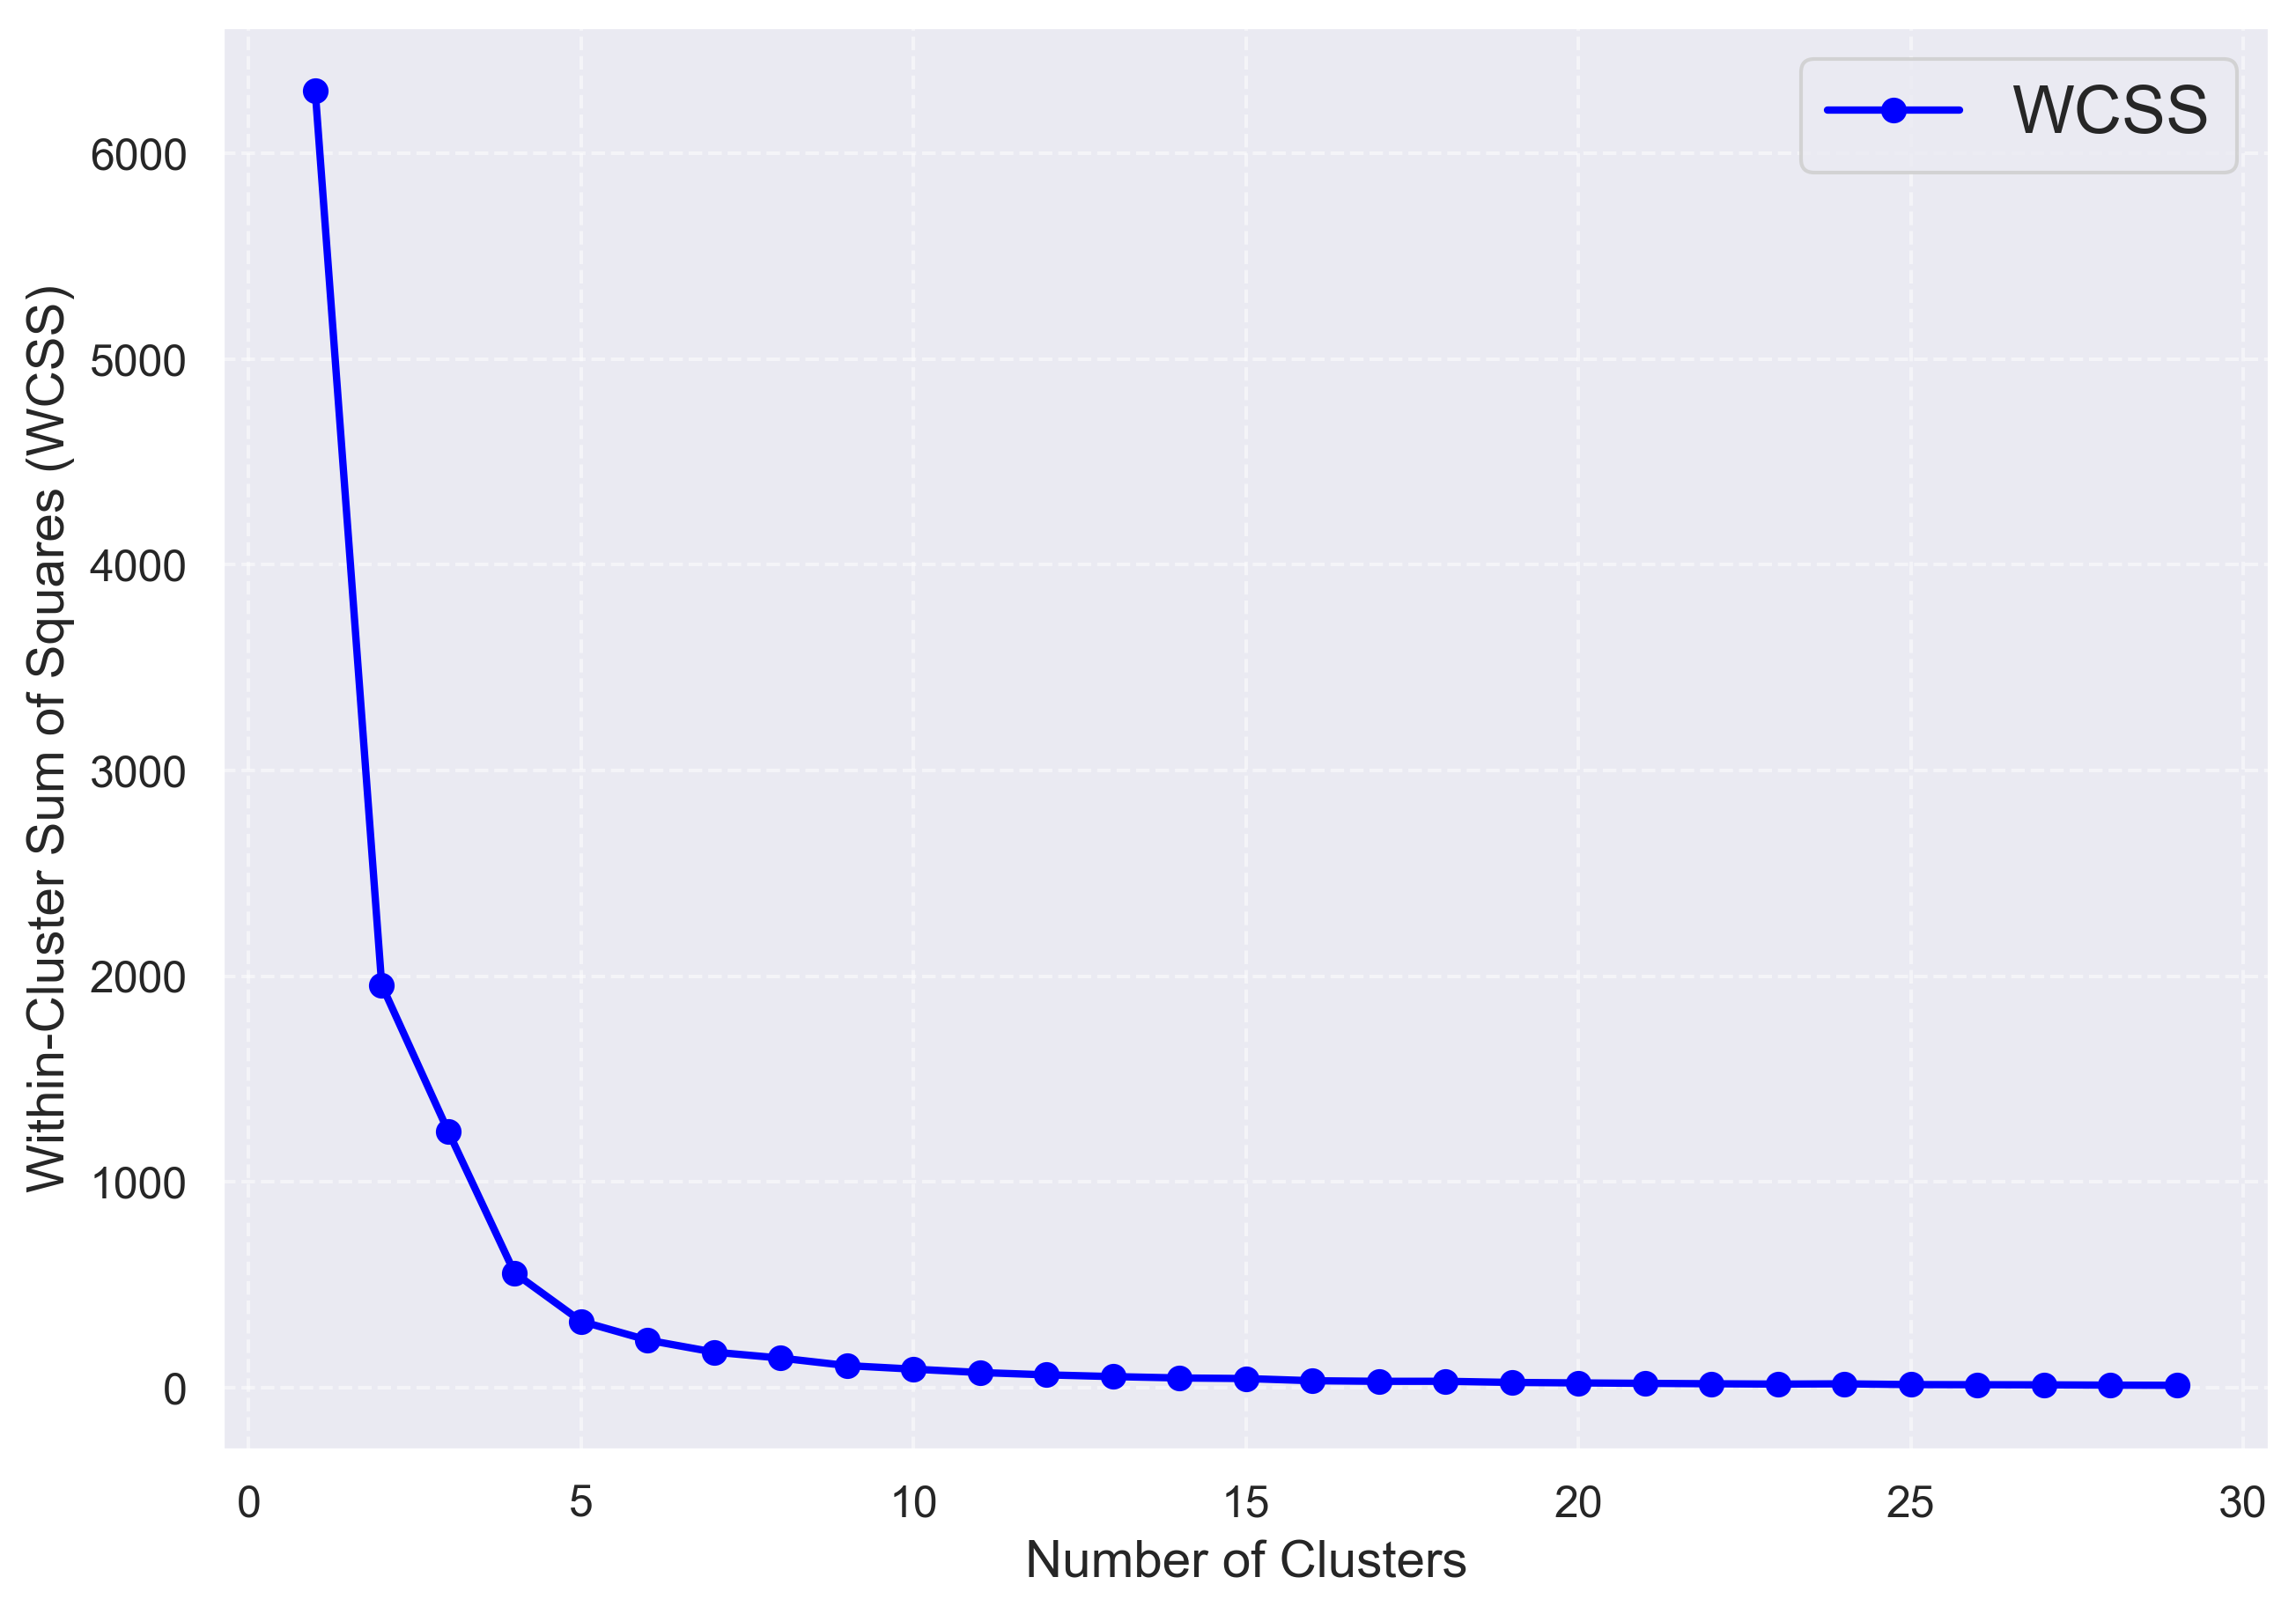
\includegraphics[width= 0.9\textwidth]{elbow.png} % Replace with your image filename
    \caption{Elbow Method for Optimal Number of Clusters}
    \label{fig:elbow} % Optional: use \label for referencing
\end{figure}


\begin{figure}[h] % 'h' places the figure approximately here
    \centering
    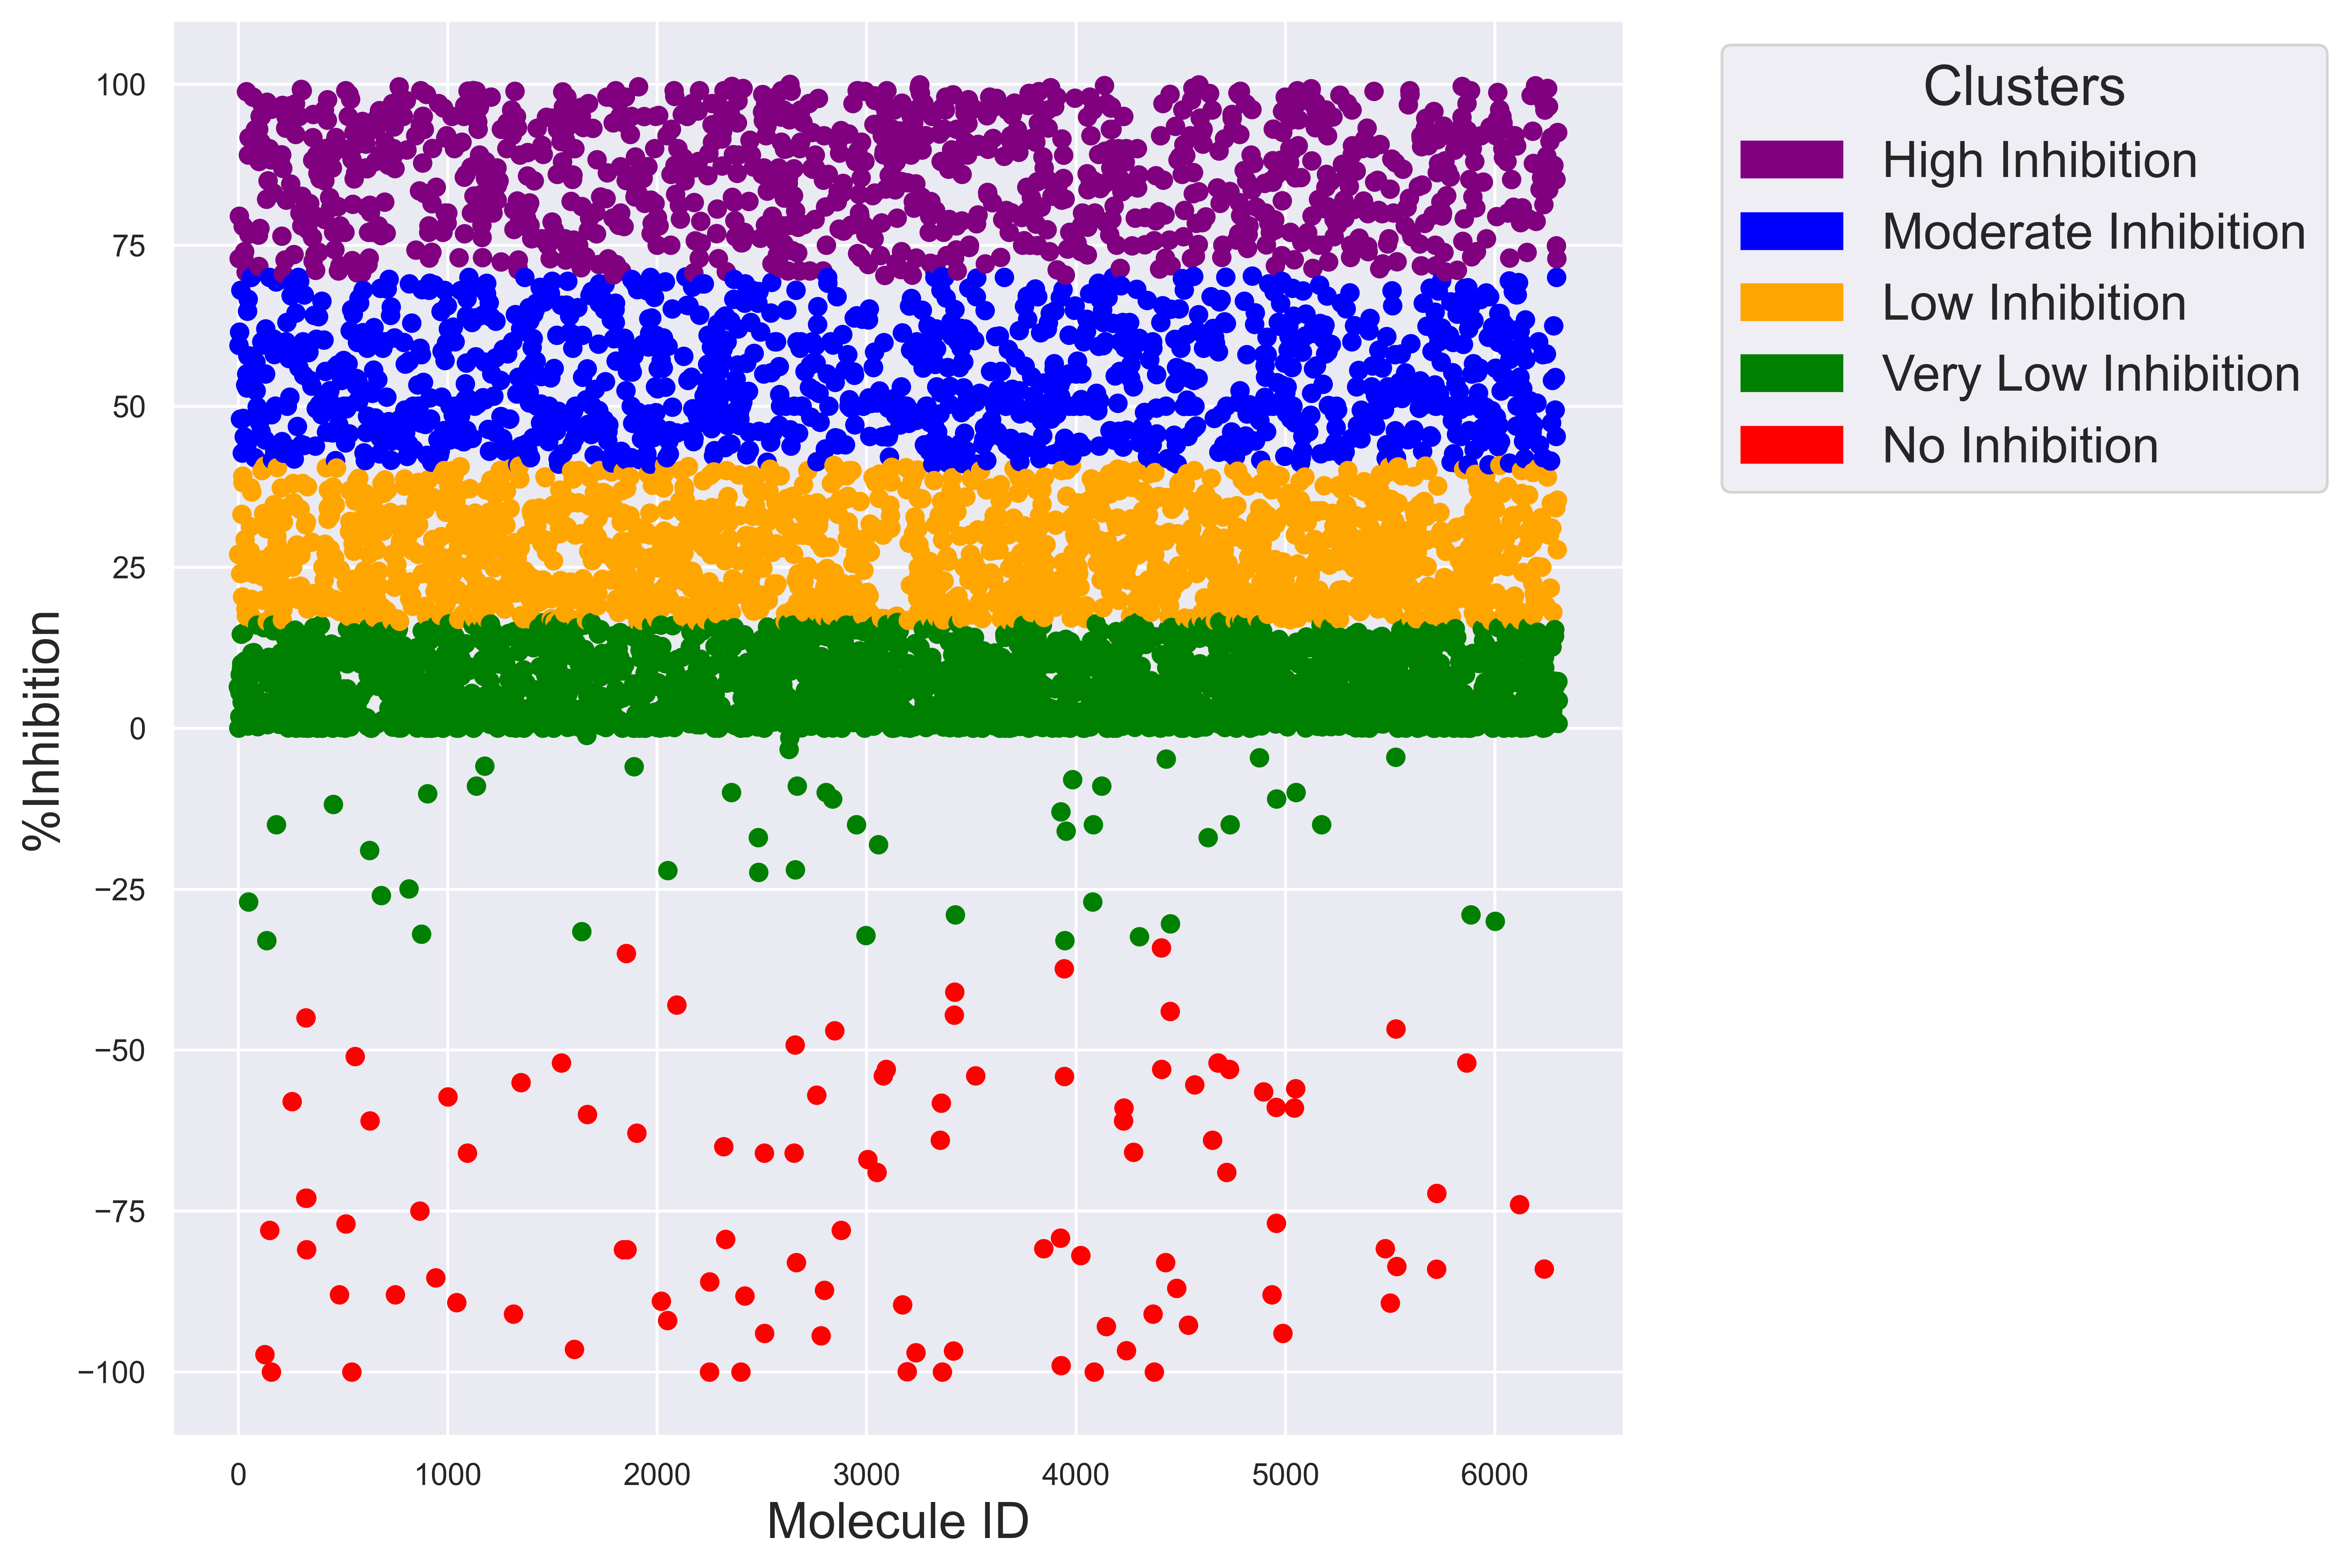
\includegraphics[scale=0.6]{cluster.png} % Replace with your image filename
    \caption{Cluster Analysis of Compounds Bioactivity Against HCT-116}
    \label{fig:cluster} % Optional: use \label for referencing
\end{figure}

HI, MI, LI, VLI and NI have the matrix dimensions of (1035 x 2048), (1162 x 2048), (1588 x 2048), (2417 x 2048), and (102 x 2048) respectively. The entire process of VLI subtraction to all categories results to a total of 9,394,879 newly formed MP's removing approximately 3,515,713 non-significant MF's. These new MP's that contain essentially the positive and negative bits were simplified by means of combining similar MP's and counting their frequencies. From this process, the positive and negative bits were identified based on their relationship with \% Inhibition against HCT-116, ranked based on frequency and compared the bits to identify commonalities. The summary of top bits is shown in \autoref{tab:bit_frequencies}. It must be noted that the resulting difference between VLI, HI and VLI, NI were considered to be positive and negative bits respectively. Whereas, the results from VLI, MI and VLI, LI difference were considered to be moderate bits. In addition, it was observed that there were common bits among the results (\autoref{fig:most_common_bits}). These findings could imply that there could be a position or neighbor dependency among the observed bits, which probably explains its presence among all the clusters.


%mentioned bits were observed on the compounds with high, moderate, low, and negative bioactivity against HCT-116. Hence, it implies that these bits could be position or neighbor dependent. This implication explains why these bits were present on the compounds with high, moderate, low and negative bioactivity. These implications can be verified through the development of CSBC-ML, wherein the input features to be used are the bits generated from CSBC.



Almost most of the common bits were found to be corresponding to small molecular fingerprints(\autoref{fig:mostcombits}). A close inspection of these bits offer some interesting observations. For instance, bit 857 and 428, are mirror images of each other, and are non-superimposable, reavealing that they are enantiomers. In addition, bits (1155, 2039), (1863, 1917) are constitutional and functional isomers. This small detail of change in conformation, connectivity and functional groups where detected through the use of CSBC method. Hence, it is expected that it will have different weights when used in CSBC-ML. 
%Observing the structures of bits 857 and 428, notice they are mirror images of each other,however,they are non-superimposable, hence they are enantiomers. In addition, bits (1155, 2039), (1863, 1917) are constitutional and functional isomers.This small detail of change in conformation, connectivity and functional groups where detected through the use of CSBC method. Therefore, when these structural features are use in the model of CSBC-ML, it is expected to have different weights.      
\FloatBarrier
\begin{figure}[h]
	\centering
	\begin{minipage}{\textwidth}
		\centering
		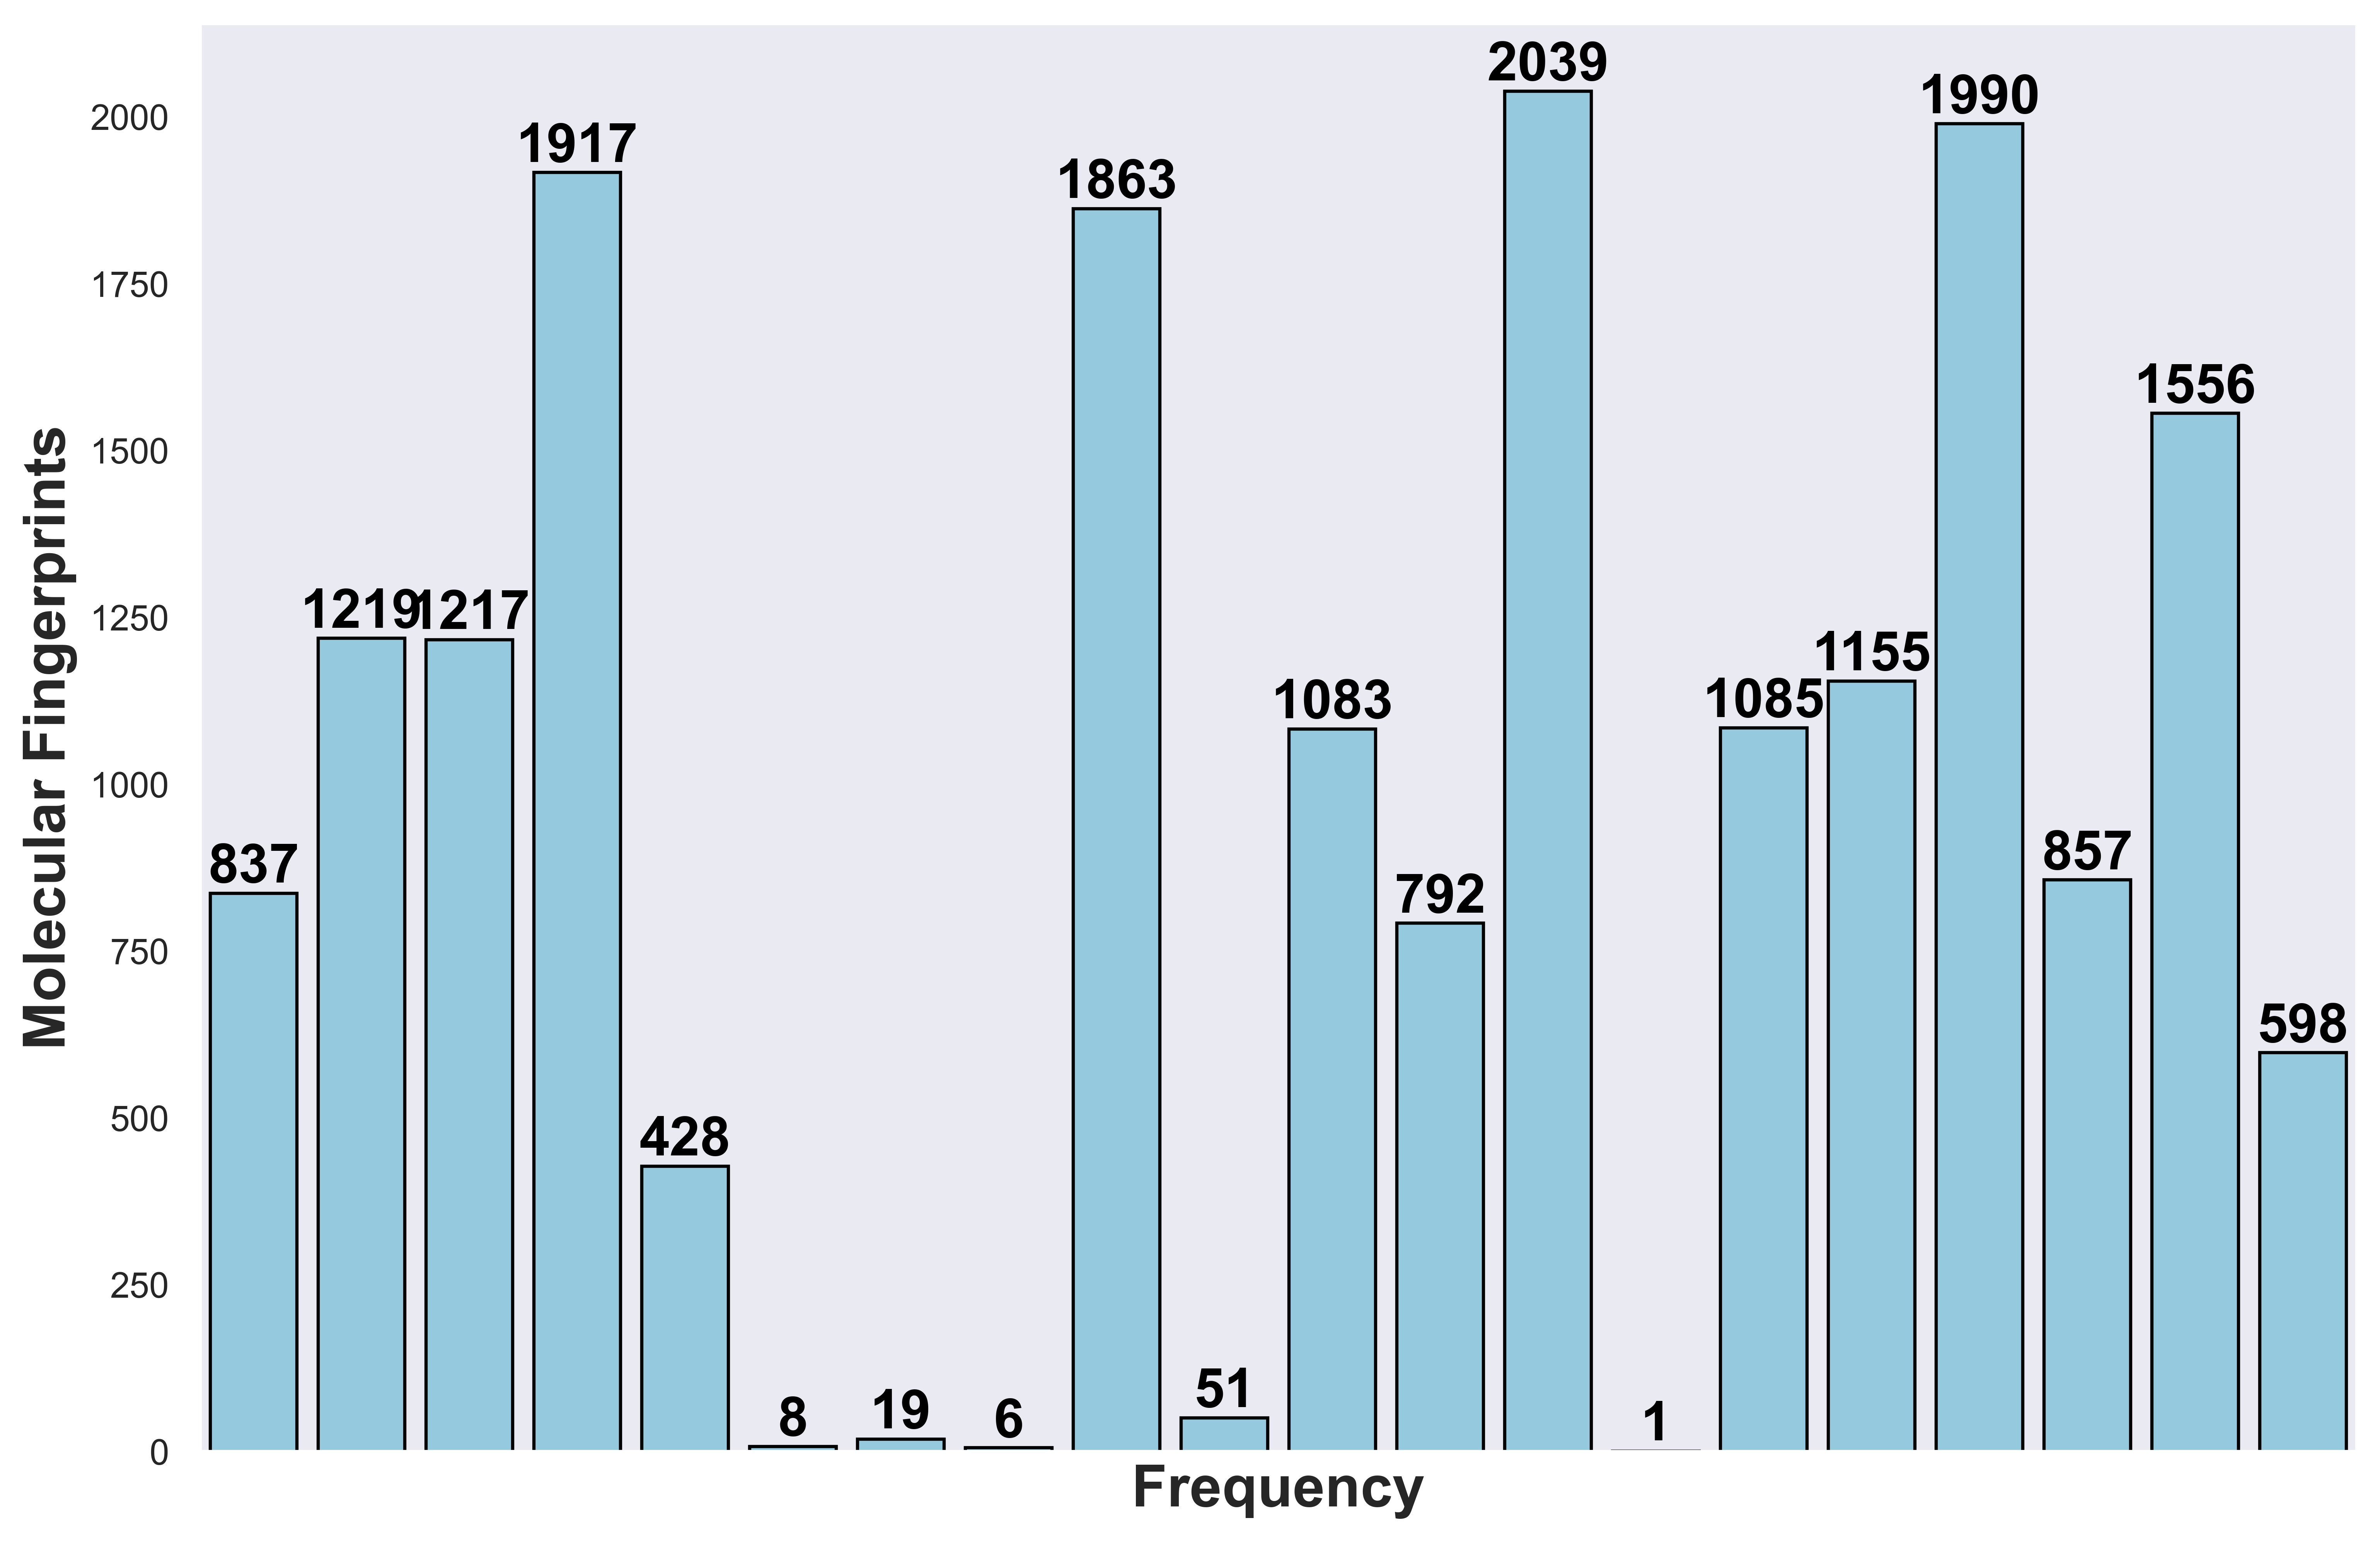
\includegraphics[width=0.8\textwidth]{bit_freq_chart.png}
		\caption{Frequently Observed Bits in different Clusters}
		\label{fig:most_common_bits}
	\end{minipage}
\end{figure}
\FloatBarrier
\begin{figure}[h]
	\centering
	\begin{minipage}{\textwidth}
		\centering
		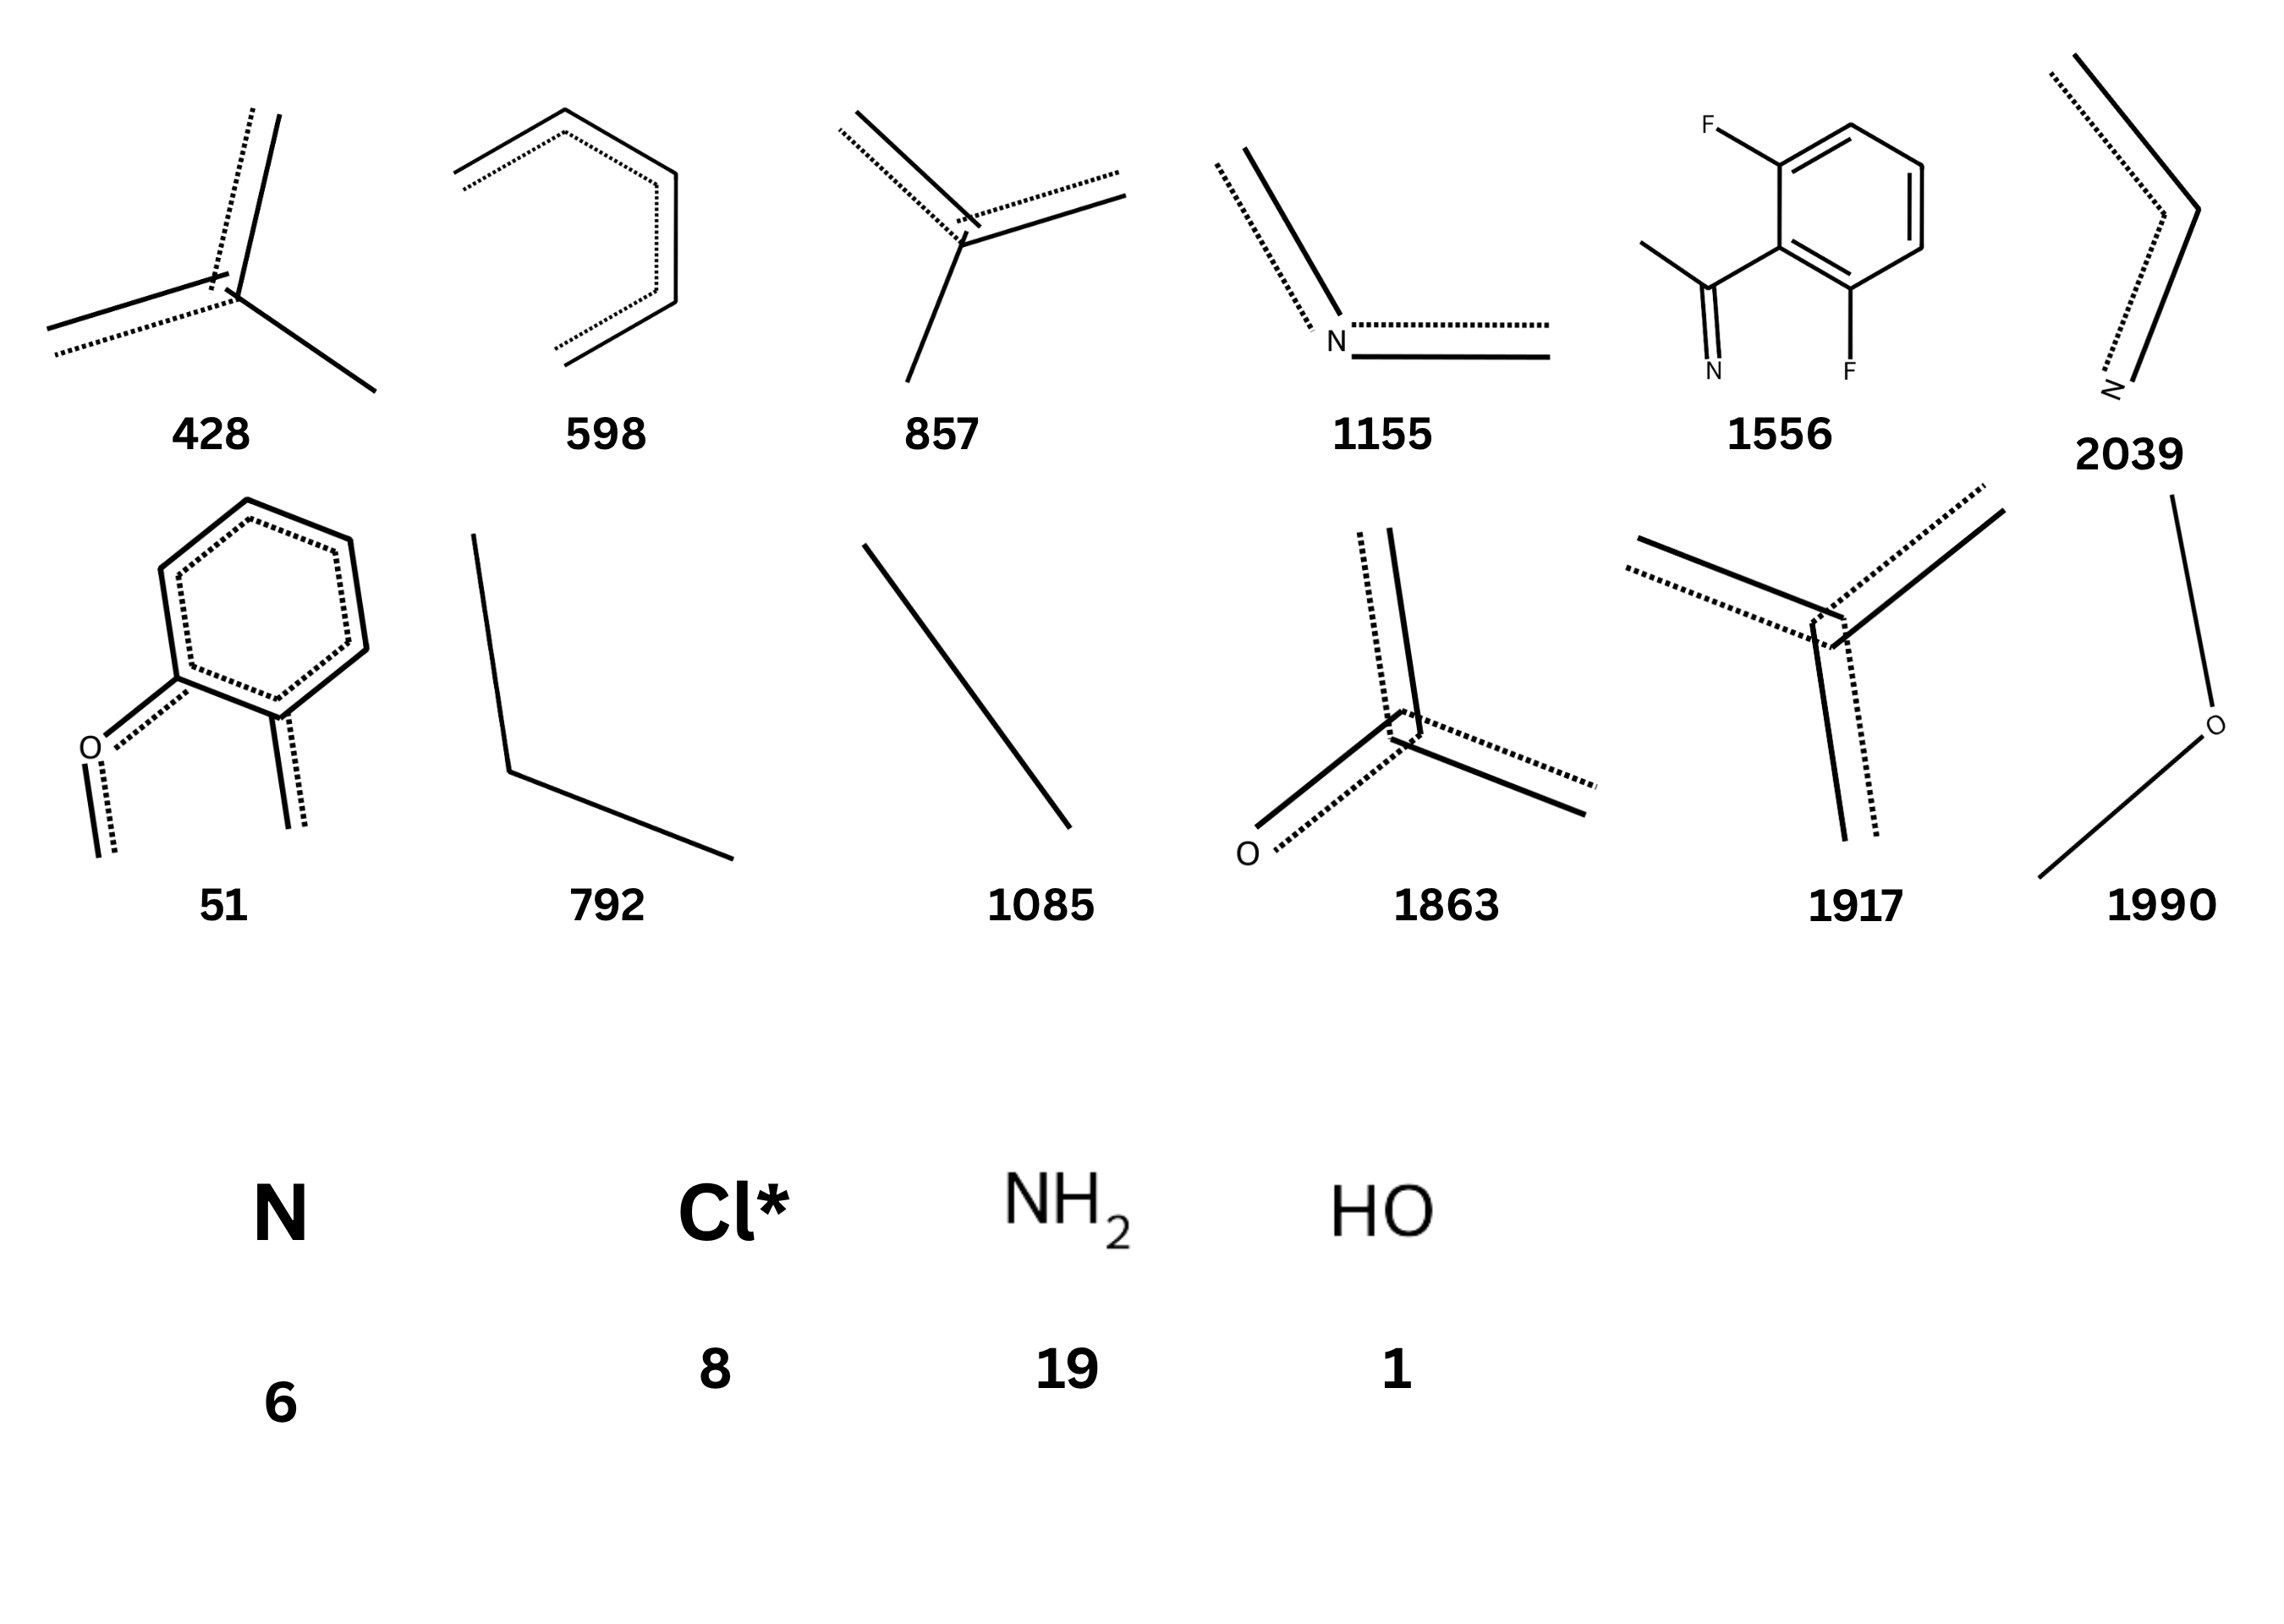
\includegraphics[width=0.8\textwidth]{mostcommonbitv2.png}
		\vspace{-0.3cm}
		
		\parbox{\textwidth}{\centering \footnotesize \textbf{*} Can be interpreted as other electronegative atoms/functional groups.}
		
		\vspace{0.3cm}
		\caption{Most Common Bits Visualization:CSBC}
		\label{fig:mostcombits}
	\end{minipage}
\end{figure}
\FloatBarrier
\subsection*{CBC-ML and CSBC-ML Development} 
%The bits extracted from CBC and CSBC methods were used as a features in the training and testing of CBC-ML and CSBC-ML. Fundamentally, it was expected that with the appropriate mathematical model, the assigned features would be enough for the machine to accurately classify the compounds activity against HCT-116. To validate these, the researchers used four mathematical models to combined with the results from structural activity relationship studies, and evaluate its performance based on confusion matrix parameters, ROC and AUC. Objectively, the researchers aimed to produce a machine learning model that have high accuracy, precision, F1 score, specificity, AUC with low FNR, FPR, and good fit between the training and testing period.  

\subsubsection*{a. Logit Model of CBC-ML and CSBC-ML}
\begin{table}[h]
\centering
\small
\renewcommand{\arraystretch}{1.2} % Adjust row spacing

\begin{tabular}{l c c}
\hline
\textbf{Metric} & \textbf{Training} & \textbf{Testing} \\
\hline
Training Accuracy & 0.7061 & 0.7092 \\
Precision         & 0.6985 & 0.6976 \\
Recall           & 0.7279 & 0.7285 \\
F1 Score         & 0.7129 & 0.7127 \\
Specificity      & 0.6842 & 0.6842 \\
False Negative Rate (FNR) & 0.2721 & 0.2721 \\
False Positive Rate (FPR) & 0.3158 & 0.3158 \\
\hline
\end{tabular}
\caption{Training and Testing Results of CSBC-ML-Logit}
\label{tab:train_test_CSBC_ML_log}
\end{table}


\begin{table}[h]
\centering
\small
\renewcommand{\arraystretch}{1.2} % Adjust row spacing

\begin{tabular}{l c c}
\hline
\textbf{Metric} & \textbf{Training} & \textbf{Testing} \\
\hline
Training Accuracy & 0.6328 & 0.6214 \\
Precision         & 0.6290 & 0.6134 \\
Recall           & 0.6519 & 0.6366 \\
F1 Score         & 0.6403 & 0.6248 \\
Specificity      & 0.6136 & 0.6136 \\
False Negative Rate (FNR) & 0.3481 & 0.3481 \\
False Positive Rate (FPR) & 0.3864 & 0.3864 \\
\hline
\end{tabular}

\caption{Training and Testing Results of CBC-ML-Logit}
\label{tab:train_test_CBC_ML_log}
\end{table}

\autoref{tab:train_test_CSBC_ML_log} to \ref{tab:train_test_CBC_ML_log} shows the summary of CSBC-ML and CBC-ML Logit based models training and testing for the classification of compounds activity or inactivity against HCT-116. Results revealed that CSBC-ML-Logit and CBC-ML-Logit during training and testing produced an accuracy of 0.7061, 0.7092, 0.6985 and 0.6976 respectively. This means that the model has enough capability to predict the compounds activity or inactivity against HCT-116. The precision values that the model produce means that it were able to correctly classify the true positive values. For the recall, results suggest that both of the models were able to identify relevant instances during the training and testing. Based on the F1 score, both of the models were able to maintain the good balance of precision and recall during the training and testing. The models appears to have a good capacity to accurately identify negative predictions. Furthermore, FNR and FPR values of the model suggest that around 30\% of the time, it would likely misclassify the true positive and negative cases \footnote{True Positive Cases:Activity Against HCT-116, True Negative Cases: Inactivity against HCT-116}. Furthermore, the ROC curve and AUC values of the models shows that TPR during the training and testing were fitted, suggesting that there is no over-fitting that takes place (\autoref{fig:roc_logit}). Overall both of the models shows a balanced performance both in training and testing, however, comparing the two, CSBC-ML-Log performs better. 
  
\begin{figure}[h] % 'h' places the figure approximately here
    \centering
    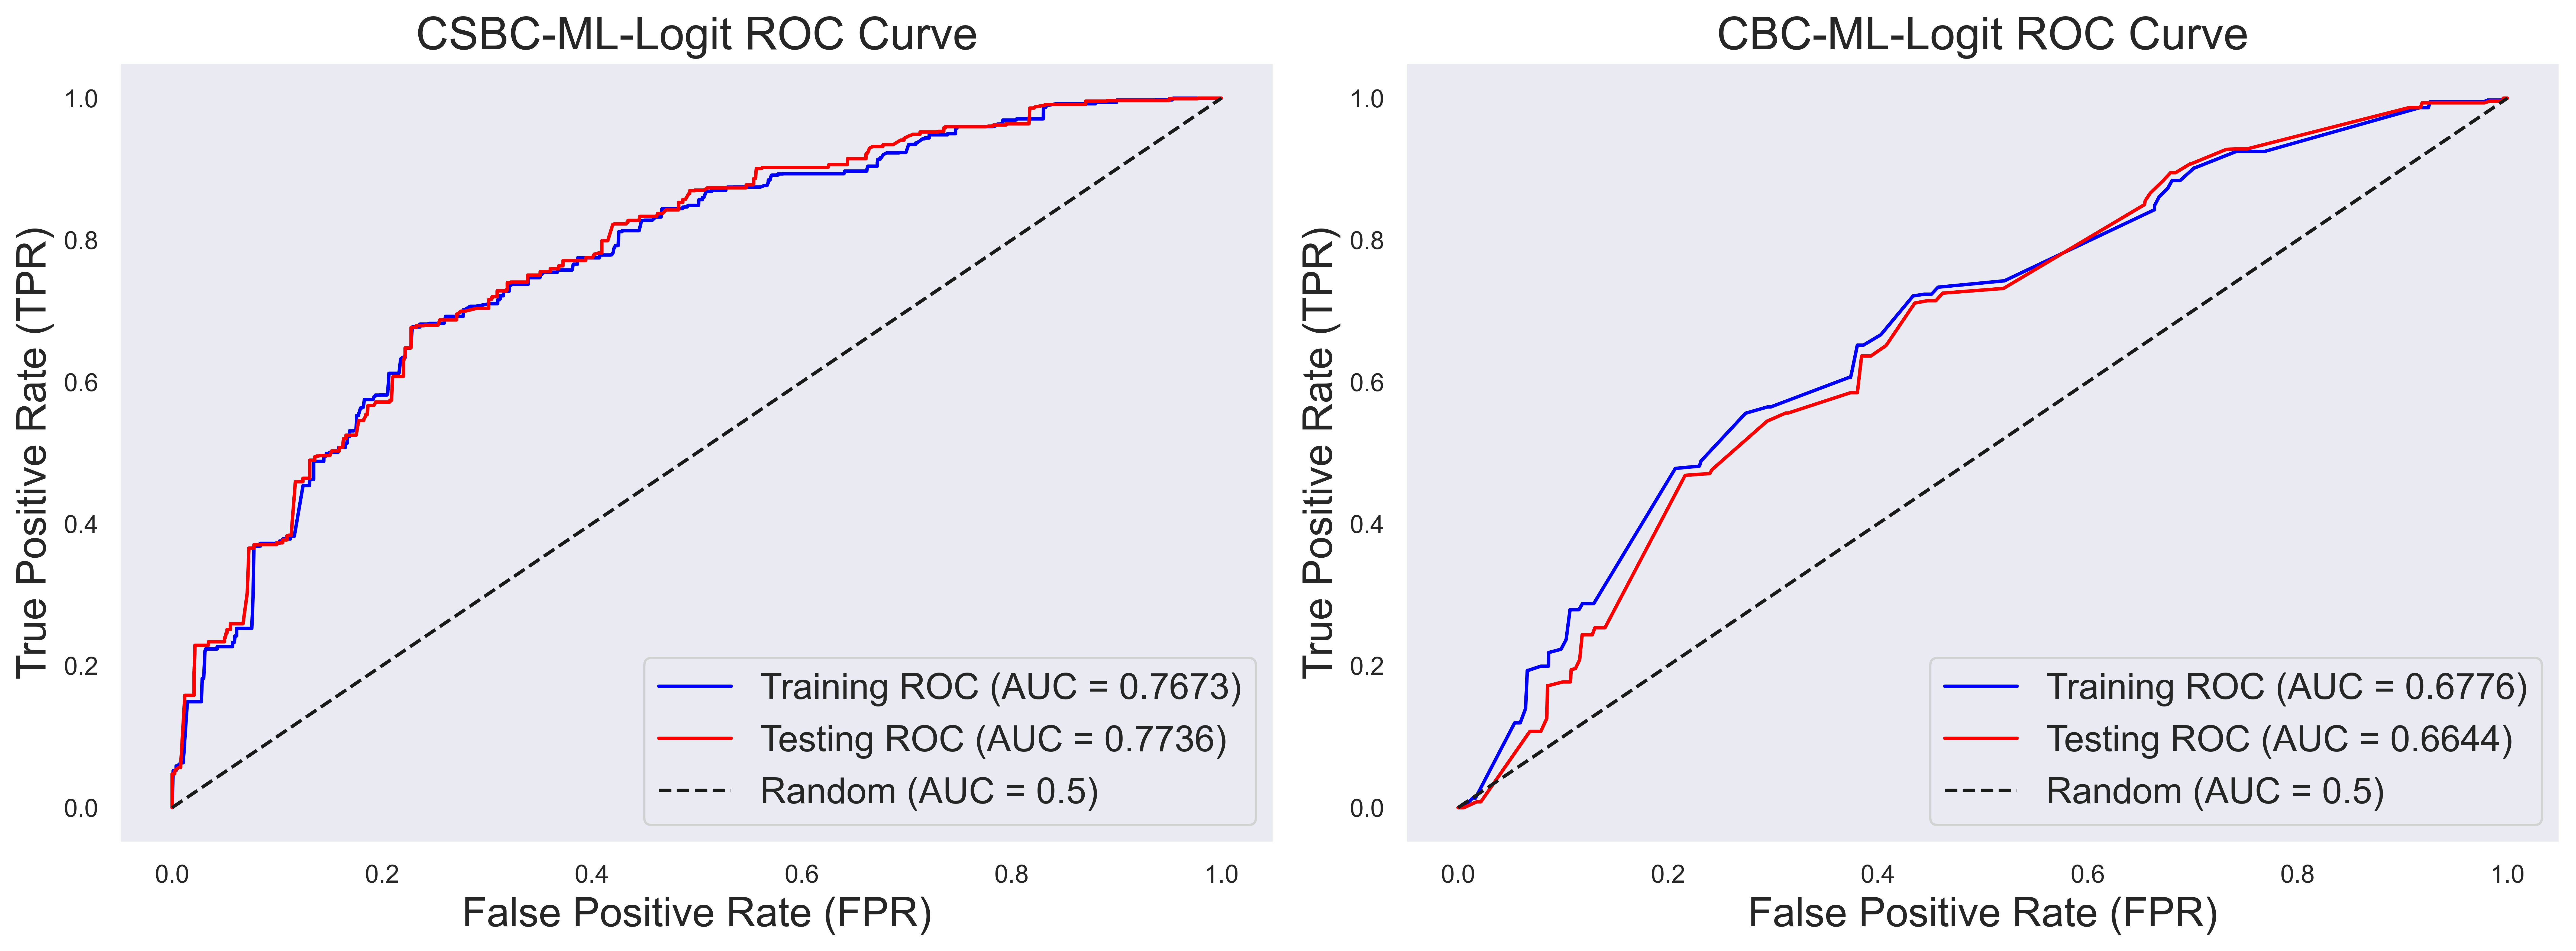
\includegraphics[scale=0.4]{combined_roc_logit.png} % Replace with your image filename
    \caption{CSBC-ML and CBC-ML Logit: Summary of ROC and AUC}
    \label{fig:roc_logit} % Optional: use \label for referencing
\end{figure}   
  
 \subsubsection*{b. XGBoost Model of CBC-ML and CSBC-ML}
For the XGBoost mathematical model of CSBC-ML and CBC-ML, results show that both of them can be classify as a good model. For CBC-ML-Xgb, the training and testing metrics revealed that: a) there is a slight decrease in accuracy, precision, and specificity --- could mean that increasing the test data could lead to more classification errors; and b) there is a slight increase in recall, and FPR --- which could imply that model has a good prediction capacity on identifying true positive cases from unseen data but needs an improvement on handling negative cases. (\autoref{tab:performance_metrics_cbc_xgb})  


%0.7299, 0.7206 accuracy, 0.7344, 0.7143 precision, 0.7222, 0.7260 recall, 0.7283, 0.7201 F1 score, 0.7376, 0.7152 specificity, 0.2778, 0.2740 FNR and 0.2624, 0.2848 FPR (\autoref{tab:performance_metrics_cbc_xgb}). 

%These results suggest the following: a) slight drops in accuracy, precision, and specificity could mean that increased in test data could lead to more classification errors; b) slight increase in recall could mean that the model has a good prediction capacity on identifying true positive cases from unseen data; and c) slight increase in FPR could mean that model needs improvement in handling negative cases. 

\begin{table}[h]
\centering
\small
\renewcommand{\arraystretch}{1.2} % Adjust row spacing

\begin{tabular}{l c c}
\hline
\textbf{Metric} & \textbf{Training} & \textbf{Testing} \\
\hline
Accuracy & 0.7299 & 0.7206 \\
Precision & 0.7344 & 0.7143 \\
Recall & 0.7222 & 0.7260 \\
F1 Score & 0.7283 & 0.7201 \\
Specificity & 0.7376 & 0.7152 \\
False Negative Rate (FNR) & 0.2778 & 0.2740 \\
False Positive Rate (FPR) & 0.2624 & 0.2848 \\
\hline
\end{tabular}

\caption{Training and Testing Performance Metrics of CBC-ML-Xgb}
\label{tab:performance_metrics_cbc_xgb}
\end{table}


\begin{table}[h]
\centering
\small
\renewcommand{\arraystretch}{1.2} % Adjust row spacing

\begin{tabular}{l c c}
\hline
\textbf{Metric} & \textbf{Training} & \textbf{Testing} \\
\hline
Accuracy & 0.9560 & 0.9488 \\
Precision & 0.9347 & 0.9240 \\
Recall & 0.9808 & 0.9770 \\
F1 Score & 0.9572 & 0.9498 \\
Specificity & 0.9312 & 0.9212 \\
False Negative Rate (FNR) & 0.0192 & 0.0230 \\
False Positive Rate (FPR) & 0.0688 & 0.0788 \\
\hline
\end{tabular}

\caption{Training and Testing Performance Metrics of CSBC-ML-Xgb}
\label{tab:performance_metrics_csbc_xgb}
\end{table}

For CSBC-ML-Xgb, both the training and testing produce very high accuracy which are 0.9560 and 0.9488 respectively. This means that, the model has a very high predicting power to classify compounds based on their structural features. Moreover, the model produce a high precision, recall, f1 score  and specificity (\autoref{tab:performance_metrics_csbc_xgb}). Although, there is a slight decrease during the training period, its value still considered to be promising. Furthermore, the model produce low FNR and FPR, suggesting that almost 99\% of the time it will be able to classify correctly the true positive and negative values. For the AUC and ROC curves of the models, both of them have value AUC $>$ 0.5, suggesting that they have a good capacity to classify the compounds. However, comparing AUC scores for training and testing of the two models, CSBC-ML-Xgb significantly outperforms CBC-ML-Xgb (\autoref{fig:roc_xgb}). 

\begin{figure}[h] % 'h' places the figure approximately here
    \centering
    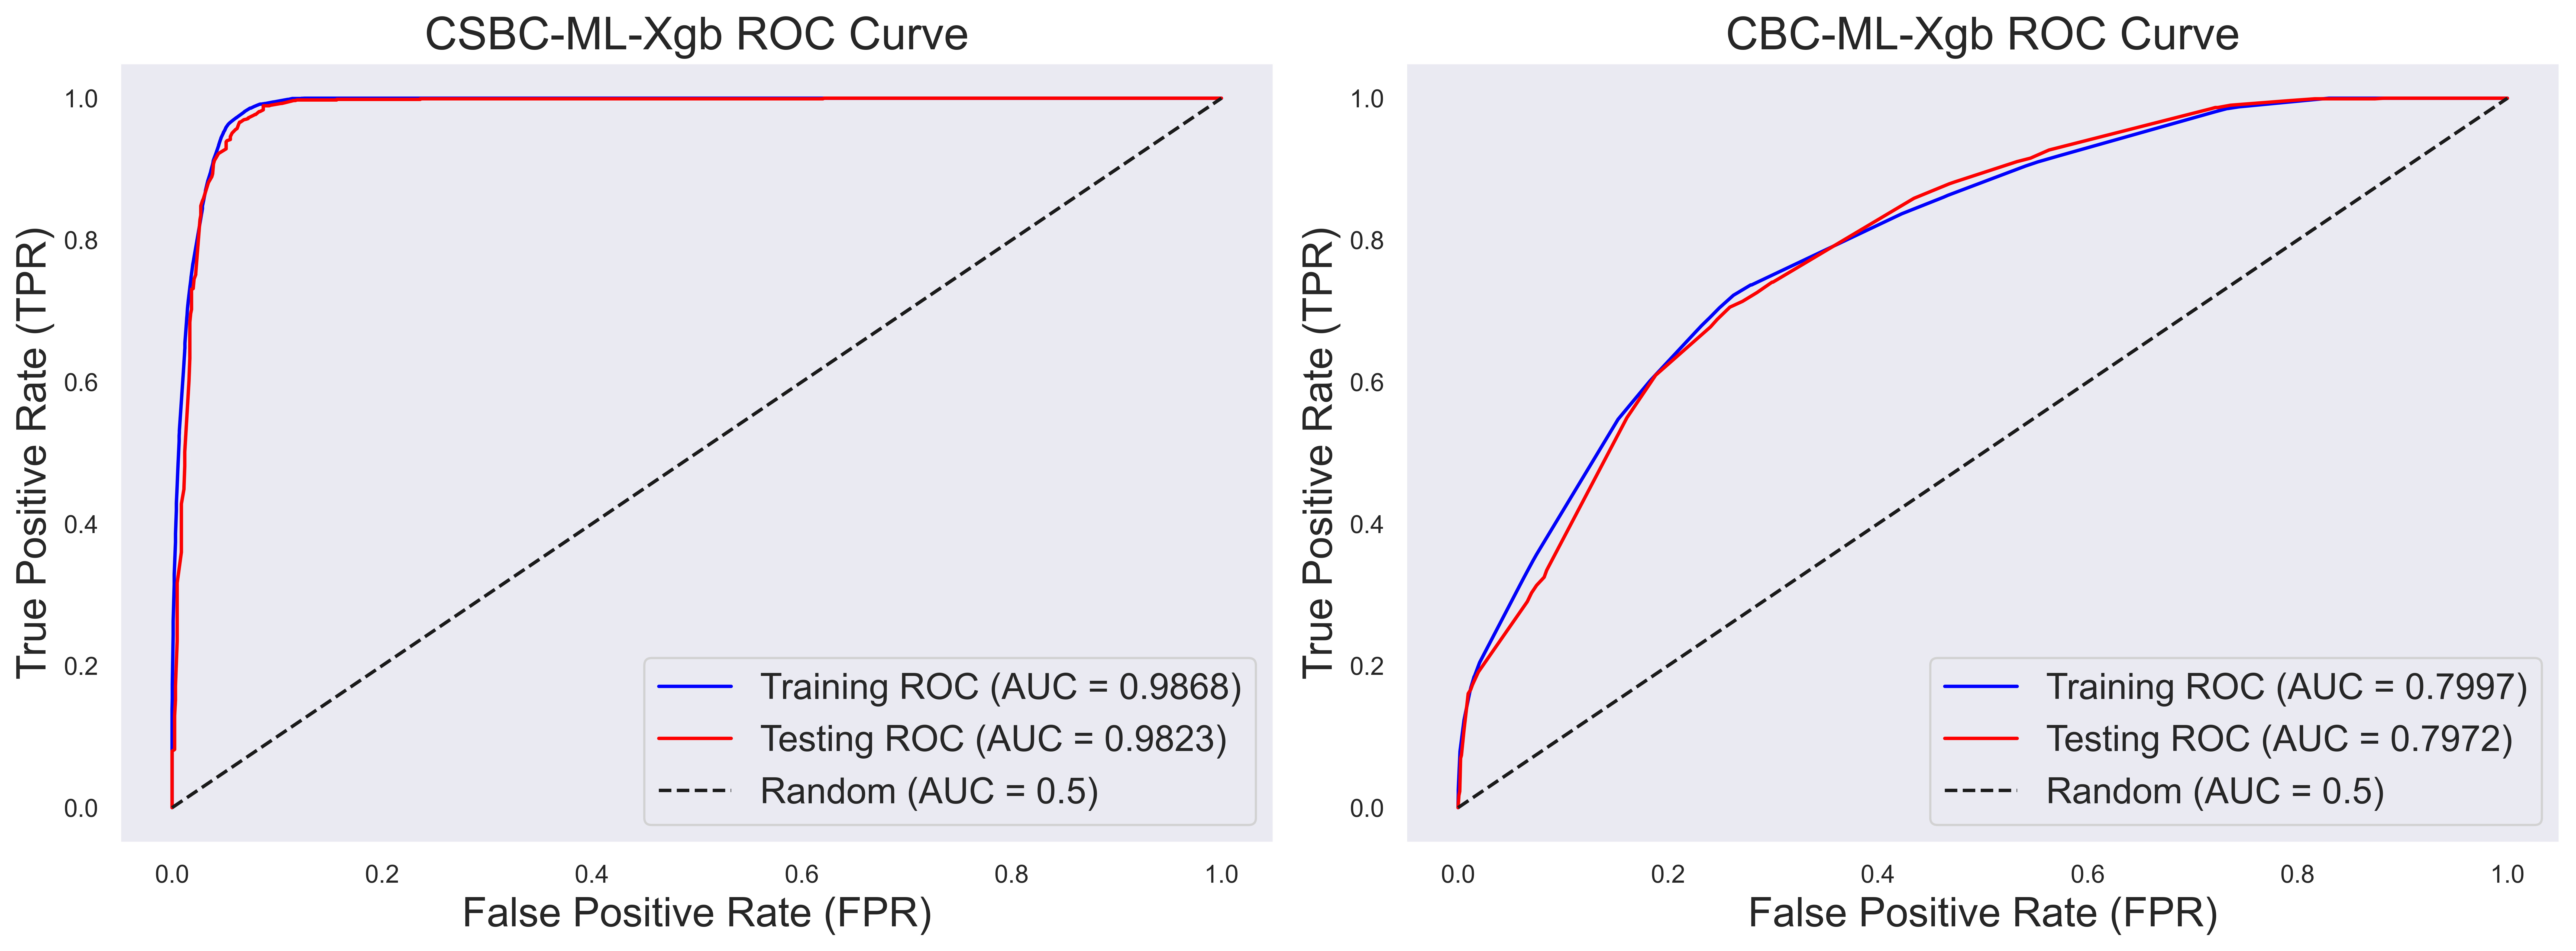
\includegraphics[scale=0.4]{combined_roc_xgb.png} % Replace with your image filename
    \caption{CSBC-ML and CBC-ML Xgb: Summary of ROC and AUC }
    \label{fig:roc_xgb} % Optional: use \label for referencing
\end{figure}

\subsubsection*{c. Random Forest Model of CBC-ML and CSBC-ML}
There is a significant difference between the CSBC-ML-RF and CBC-ML-RF in terms of confusion matrix parameters, AUC and ROC. In CSBC-ML-RF, the results shown that both in training and testing it has high accuracy, precision, recall, f1 score, and specificity. In addition, the model has low FNR, and FPR (\autoref{tab:performance_metrics_csbc_rf}). These results suggest that,  it can be identify as a good classification model with strong ability to generalize unseen data with minimal false predictions. On the other hand, CBC-ML-RF training and testing results revealed that: a) there is decrease in accuracy, precision, f1 score, and specificity --- which implies that there is a high potential misclassification that may occur if the test data increases; and b) increase in recall, FPR and slight decrease with FNR  overall affects the model's ability to classify true positive and negative values (\autoref{tab:performance_metrics_cbc_rf}). Overall, CBC-ML-RF model have a good balanced performance, but, its accuracy, precision, specificity, recall, and f1 score were expected to decrease when the test data increases. Considering these findings, CSBC-ML-RF significantly outperforms CBC-ML-RF model.    

\begin{table}[h]
\centering
\small
\renewcommand{\arraystretch}{1.2} % Adjust row spacing

\begin{tabular}{l c c}
\hline
\textbf{Metric} & \textbf{Training} & \textbf{Testing} \\
\hline
Accuracy & 0.9562 & 0.9484 \\
Precision & 0.9348 & 0.9233 \\
Recall & 0.9812 & 0.9770 \\
F1 Score & 0.9574 & 0.9494 \\
Specificity & 0.9312 & 0.9204 \\
False Negative Rate (FNR) & 0.0188 & 0.0230 \\
False Positive Rate (FPR) & 0.0688 & 0.0796 \\
\hline
\end{tabular}

\caption{Training and Testing Performance Metrics of CSBC-ML-RF}
\label{tab:performance_metrics_csbc_rf}
\end{table}

\begin{table}[h]
\centering
\small
\renewcommand{\arraystretch}{1.2} % Adjust row spacing

\begin{tabular}{l c c}
\hline
\textbf{Metric} & \textbf{Training} & \textbf{Testing} \\
\hline
Accuracy & 0.7300 & 0.7206 \\
Precision & 0.7346 & 0.7143 \\
Recall & 0.7222 & 0.7260 \\
F1 Score & 0.7284 & 0.7201 \\
Specificity & 0.7378 & 0.7152 \\
False Negative Rate (FNR) & 0.2778 & 0.2740 \\
False Positive Rate (FPR) & 0.2622 & 0.2848 \\
\hline
\end{tabular}

\caption{Training and Testing Performance Metrics of CBC-ML-RF}
\label{tab:performance_metrics_cbc_rf}
\end{table}

The AUC and ROC of the two models shows that CSBC-ML-RF has a good fit and high AUC value compared to CBC-ML-RF. Both of the models shows no signs of over-fitting based on their ROC curve (\autoref{fig:roc_rf}).


%it was drawn that the features extracted from the CSBC were more effective than CBC method. Furthermore, due to its performance (together with CSBC-ML-Xgb), it is considered to be shortlisted in the final machine model to be used in in vitro screening of drug molecules against HCT-116. 

\begin{figure}[H] % 'h' places the figure approximately here
    \centering
    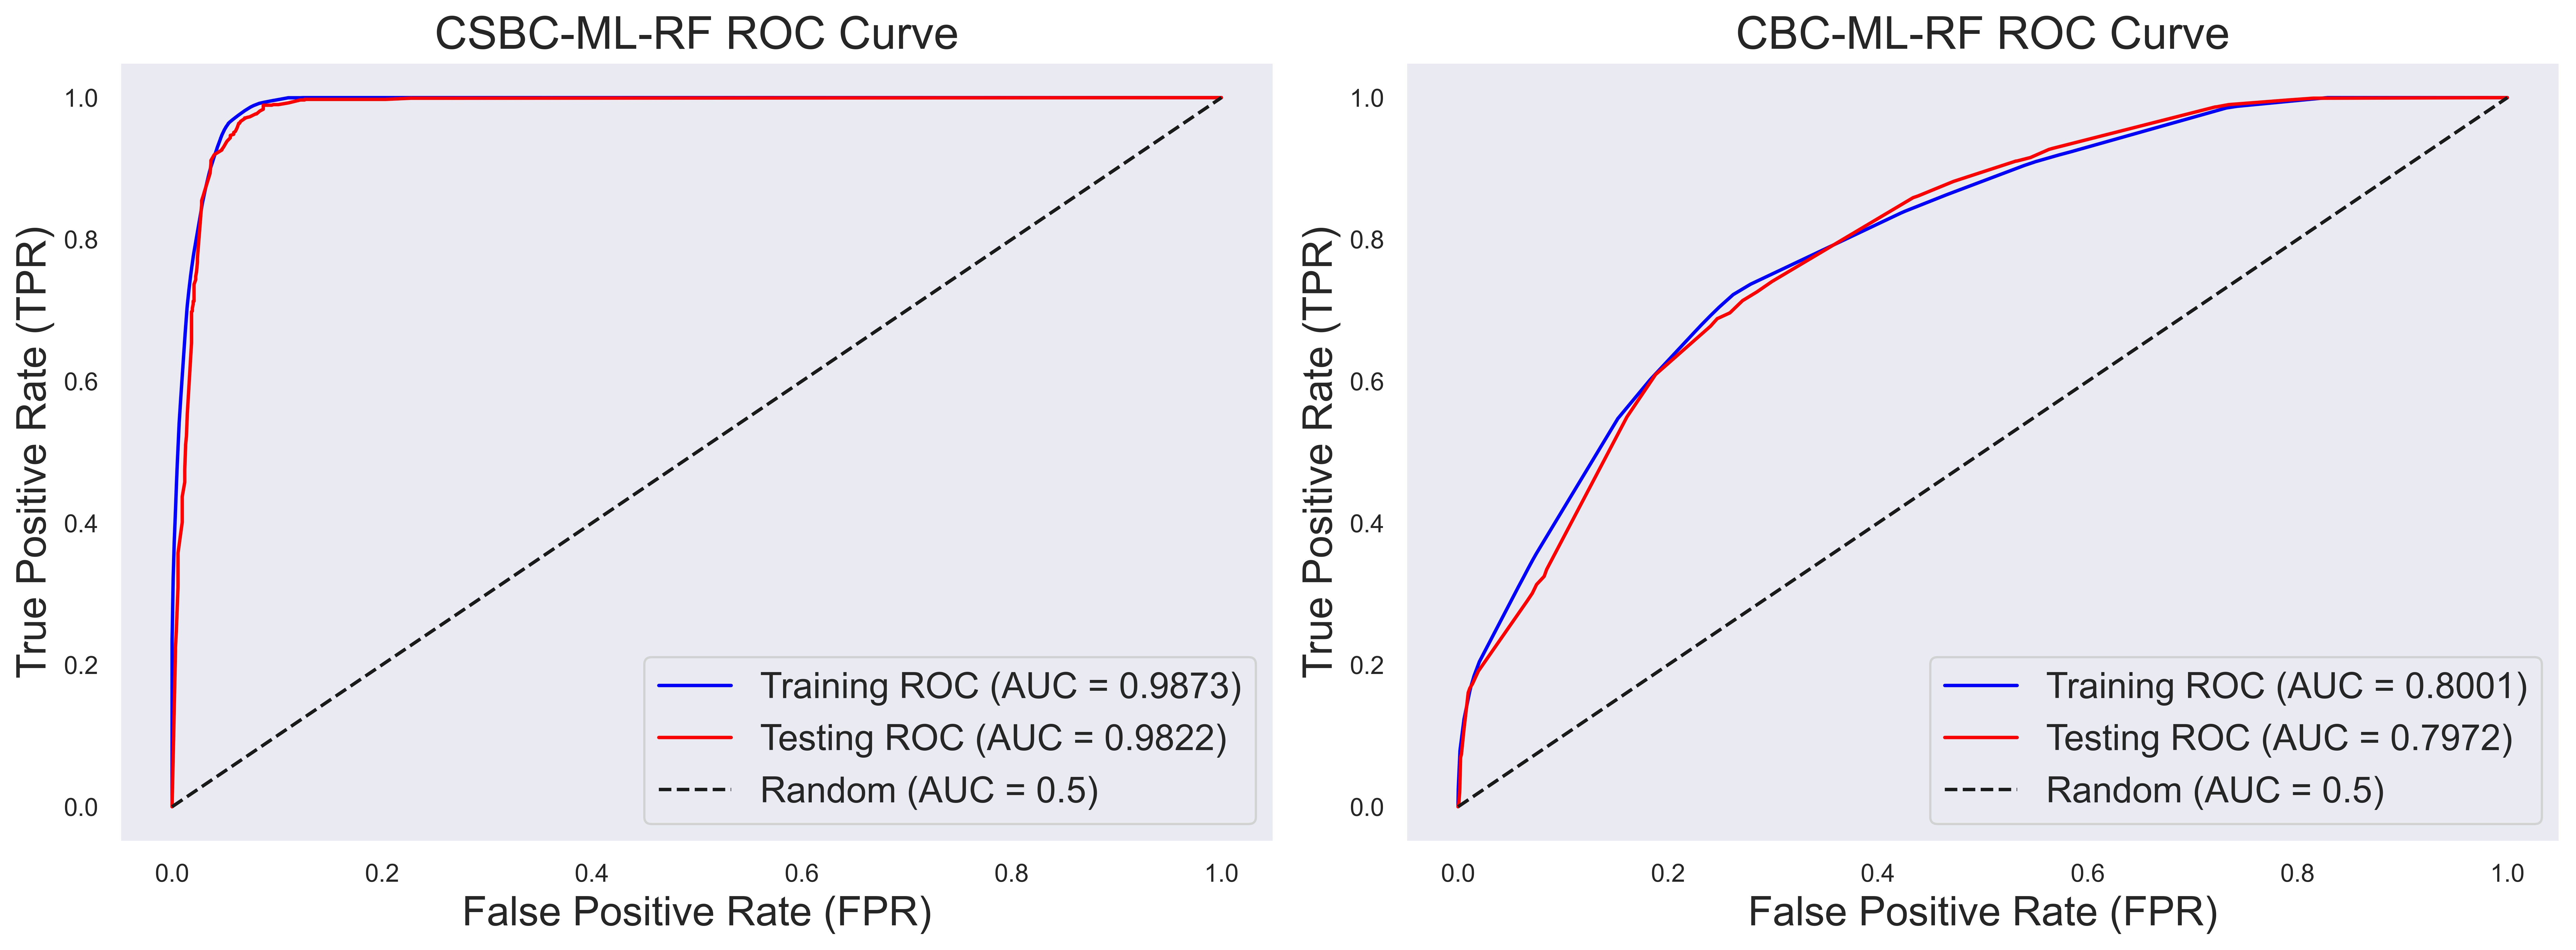
\includegraphics[scale=0.4]{combined_roc_rf.png} % Replace with your image filename
    \caption{CSBC-ML and CBC-ML RF: Summary of ROC and AUC }
    \label{fig:roc_rf} % Optional: use \label for referencing
\end{figure}

\subsubsection*{d. Support Vector Machine Model of CBC-ML and CSBC-ML}

\begin{table}[h]
\centering
\small
\renewcommand{\arraystretch}{1.2} % Adjust row spacing

\begin{tabular}{l c c}
\hline
\textbf{Metric} & \textbf{Training} & \textbf{Testing} \\
\hline
Accuracy & 0.9476 & 0.9435 \\
Precision & 0.9283 & 0.9239 \\
Recall & 0.9704 & 0.9655 \\
F1 Score & 0.9489 & 0.9442 \\
Specificity & 0.9247 & 0.9220 \\
False Negative Rate (FNR) & 0.0296 & 0.0345 \\
False Positive Rate (FPR) & 0.0753 & 0.0780 \\
\hline
\end{tabular}

\caption{Training and Testing Performance Metrics of CSBC-ML-SVM}
\label{tab:performance_metrics_csbc_svm}
\end{table}


Findings in CSBC-ML-SVM reveals that the accuracy, precision, recall, f1 score, specificity, FNR, and FPR does not significantly change (\autoref{tab:performance_metrics_csbc_svm}). These results indicates that the model retains its good performance even when exposed to unseen data. Overall, the high values of confusion matrix parameters suggest that the produced model is excellent on classifying compounds activity or inactivity against HCT-116. Whereas, CBC-ML-SVM results shows significant decrease in confusion matrix parameters. This suggest that the model predictions would often lead to misclassifications of true negative values. (\autoref{tab:performance_metrics_cbc_svm}).   
\vspace{-0.5cm}
\begin{table}[h]
\centering
\small
\renewcommand{\arraystretch}{1.2} % Adjust row spacing

\begin{tabular}{l c c}
\hline
\textbf{Metric} & \textbf{Training} & \textbf{Testing} \\
\hline
Accuracy & 0.7300 & 0.7206 \\
Precision & 0.7346 & 0.7143 \\
Recall & 0.7222 & 0.7260 \\
F1 Score & 0.7284 & 0.7201 \\
Specificity & 0.7378 & 0.7152 \\
False Negative Rate (FNR) & 0.2778 & 0.2740 \\
False Positive Rate (FPR) & 0.2622 & 0.2848 \\
\hline
\end{tabular}
\caption{Training and Testing Performance Metrics of CBC-ML-SVM}
\label{tab:performance_metrics_cbc_svm}
\end{table}

\FloatBarrier
\begin{figure}[h] % 'h' places the figure approximately here
    \centering
    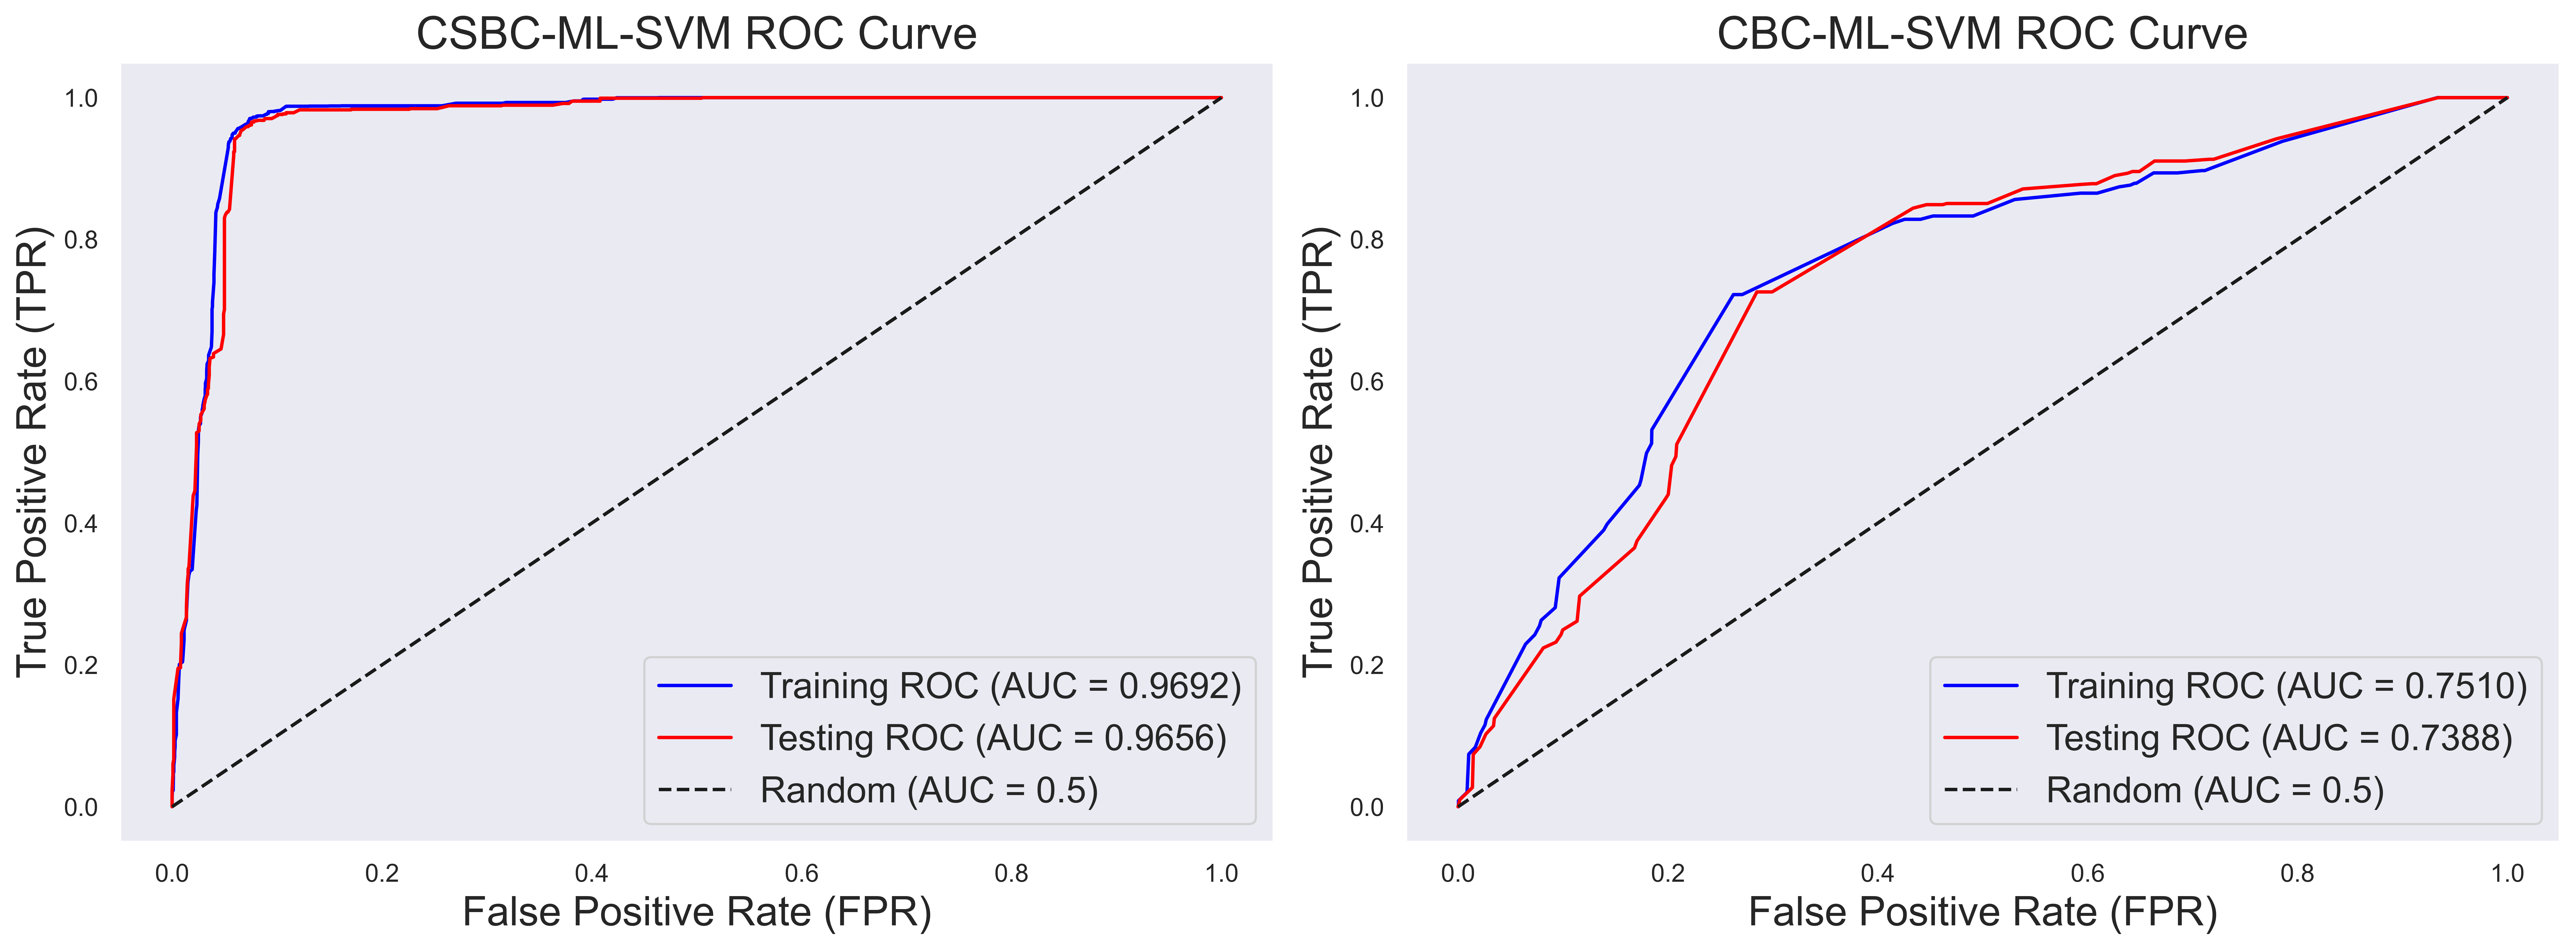
\includegraphics[scale=0.4]{combined_roc_svm.png} % Replace with your image filename
    \caption{CSBC-ML and CBC-ML SVM: Summary of ROC and AUC }
    \label{fig:roc_svm} % Optional: use \label for referencing
\end{figure}
\FloatBarrier

Analyzing the overall performance of the models shows that CSBC-ML-SVM produce high AUC's scores and it does not significantly change during the testing period. For the ROC curve, training and testing almost perfectly overlaps, suggesting that over-fitting was not observed. For CBC-ML-SVM, AUC scores can be considered good, however, ROC curves of training and testing does not perfectly overlap --- which might lead to over-fitting. Thus, CSBC-ML-SVM significantly outperforms CBC-ML-SVM.

%which could mean that it might deviate further if the test data increases, thus, might leads  to over-fitting.
\subsubsection*{e. Comparative Analysis of All QSAR-ML Models}

\begin{figure}[h] % 'h' places the figure approximately here
    \centering
    \includegraphics[scale=0.4]{model_comparison_collage.png} % Replace with your image filename
    \caption{Comparative Summary of CSBC-ML and CBC-ML}
    \label{fig:model_comparison} % Optional: use \label for referencing
\end{figure}

To evaluate the performance of all the QSAR-ML models, the confusion matrix parameters and the AUC scores were compared. Results show the following observations: a) in terms of accuracy, recall, F1 and AUC scores all of CSBC-ML models out performs CBC-ML; b) Logit based model of CSBC-ML and CBC-ML are the least performing; c) the accuracy, recall, f1 and AUC score of XGB, RF and SVM based model of CSBC-ML were not significantly different; and d) the best QSAR-ML models for classifying activity or inactivity of molecules against HCT-116 are the CSBC-ML-Xgb, CSBC-ML-RF and CSBC-ML-SVM.(\autoref{fig:model_comparison} to \autoref{fig:model_comparison_auc}).       

\begin{figure}[h] % 'h' places the figure approximately here
    \centering
    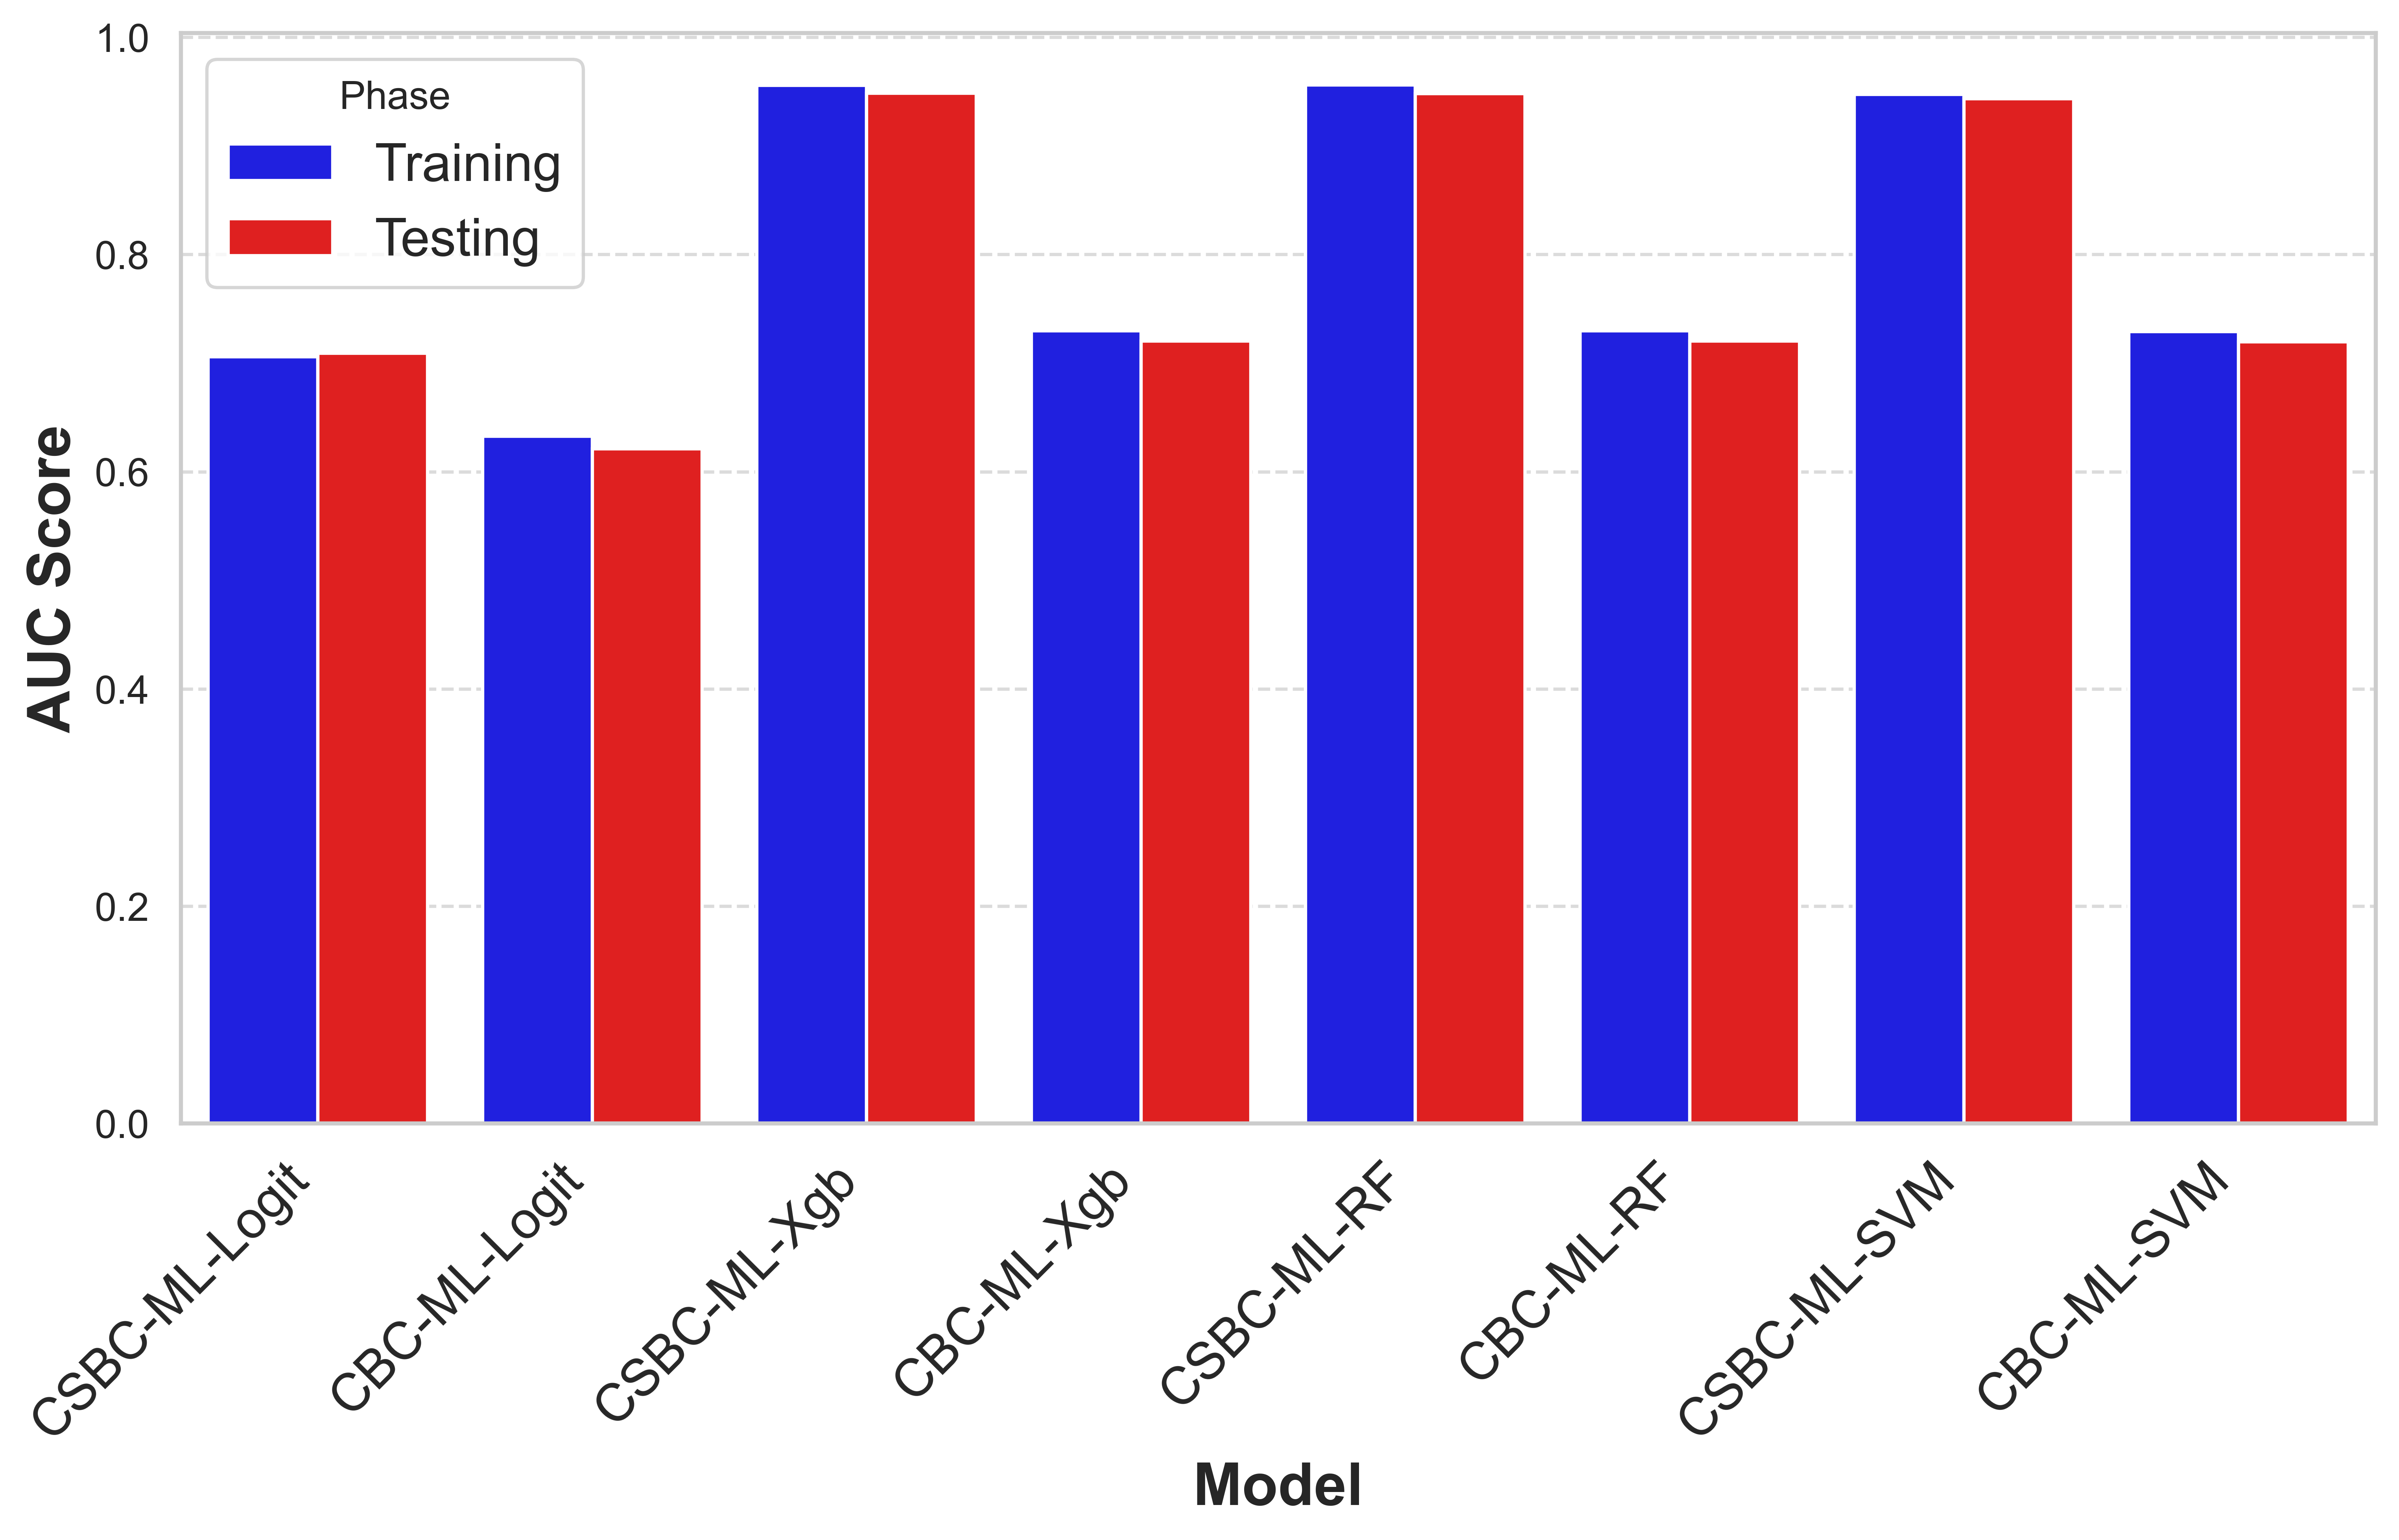
\includegraphics[scale=0.6]{auc_comparison.png} % Replace with your image filename
    \caption{Comparative Summary of CSBC-ML and CBC-ML: AUC Scores}
    \label{fig:model_comparison_auc} % Optional: use \label for referencing
\end{figure}

Based from these findings, it was identified that CSBC-ML-Xgb, CSBC-ML-RF and CSBC-ML-SVM were the best candidates to proceed in the development of in vitro virtual drug screening MLA. Moreover, at this point, it clear that bit features extracted from the CSBC method were better than CBC. This was confirmed when all of the CSBC-ML models outperforms CBC-ML, hence, the creation of CSBC-ML method were proven to be effective. Finally, the over-simplification in CBC method generation of bits, takes its toll when combined with different mathematical models.  